%\documentclass[onecolumn]{aa} % for a paper on 1 column  
%\documentclass[longauth]{aa} % for the long lists of affiliations
%\documentclass[bibyear]{aa} % if the references are not structured according to the author-year natbib style
%\documentclass{aa}  
%\documentclass{memoir}
%\documentclass[oldfontcommands]{memoir}
%\documentclass[twocolumn]{revtex4-2}
%\documentclass[12pt,a4paper,oldfontcommands]{memoir}
\documentclass[10pt,a4paper]{article}
%\documentclass[10pt,a4paper,onecolumn]{paper}
\usepackage{fullpage}

\usepackage{amsmath}
\usepackage{amssymb}
\usepackage{graphicx}
%\usepackage{txfonts}
\usepackage[linktocpage=true, colorlinks=true, allcolors=blue]{hyperref}
\usepackage[labelfont=bf]{caption}
\usepackage[noabbrev]{cleveref}
\usepackage{tensor}
\usepackage{derivative}
\usepackage{booktabs}
\usepackage{mathtools}
\usepackage[export]{adjustbox}

\usepackage{biblatex}
%\bibliographystyle{plainnat}
\addbibresource{report.bib}

\newcommand\TODO[1]{\textcolor{red}{(\textbf{TODO:} #1)}}
\DeclareMathOperator{\asin}{asin}
\DeclareMathOperator{\sinc}{sinc}
\DeclareMathOperator{\diag}{diag}
\DeclareMathOperator{\argmax}{argmax}
%\setlength{\mathindent}{20pt}

\begin{document}

\title{\textbf{Solving the Einstein-Boltzmann equations}\\ \\\normalsize\textit{(AST5220 project report)}}
%\subtitle{Einstein-Boltzmann solver}
\author{Herman Sletmoen}

%\institute{ITA Oslo}
\date{Spring 2023}

\iffalse
\abstract
% context heading (optional)
{Solve Einstein-Boltzmann equations}
% aims heading (mandatory)
{Solve Einstein-Boltzmann equations}
% methods heading (mandatory)
{Solve Einstein-Boltzmann equations}
% results heading (mandatory)
{Solve Einstein-Boltzmann equations}
% conclusions heading (optional)
{Solve Einstein-Boltzmann equations}
\fi

%\keywords{cosmology -- Einstein-Boltzmann equations}

\maketitle
\tableofcontents
%
%________________________________________________________________

%\tableofcontents

\bigskip \bigskip \bigskip

\noindent
\textbf{Code:}
All code is available at \href{https://github.com/hersle/AST5220-project}{https://github.com/hersle/AST5220-project}.
I chose to implement this project from scratch in Julia,
as it is an interesting programming language I wanted to learn more about.

\clearpage

\setcounter{section}{-1}
\section{Introduction}
\label{sec_intro}

The goal of this project is to theoretically predict
power spectra for matter and the cosmic microwave background (CMB).
This essentially involves solving the \textbf{Einstein field equations}
\begin{equation}
	G\indices{_\mu_\nu} + \Lambda g\indices{_\mu_\nu} = \frac{8 \pi G}{c^4} T\indices{_\mu_\nu},
\label{eq_einstein}
\end{equation}
where the distribution function $f_s(\mathbf{x},\mathbf{p},t)$ for different species $s$
gives rise to the total energy-momentum
\begin{equation}
	T\indices{^\mu_\nu}(\mathbf{x},t) = \sum_s \frac{g_s}{\sqrt{-|g|}} \int \frac{dP_1 dP_2 dP_3}{(2\pi\hbar)^3} \frac{P^\mu P_\nu}{P^0} f_s(\mathbf{x},\mathbf{p},t),
\label{eq_energy_momentum}
\end{equation}
and the distribution function evolves according to the \textbf{Boltzmann equation}
\begin{equation}
	\frac{df_s}{dt} = \frac{\partial f_s}{\partial t} + \frac{\partial f_s}{\partial x^i} \frac{dx^i}{dt} + \frac{\partial f_s}{\partial p^i} \frac{d p^i}{dt} = C[f_s],
\label{eq_boltzmann}
\end{equation}
and the collision term $C[f_s]$ describes how
elements of the distribution function move in phase space
due to interactions (or ``collisions'') between particles.
A computer program that solves these equations
is commonly referred to as an \emph{Einstein-Boltzmann solver}.

We begin by
solving the background FLRW cosmology in \cref{sec_background_cosmology}
and recombination and reionization history in \cref{sec_recombination}.
In \cref{sec_perturbations} we find their first-order linear perturbations in Fourier-space.
Finally, in \cref{sec_power_spectra}, we combine everything
to compute the power spectra of matter in Fourier-space
and of the CMB projected on a sphere with spherical harmonics.

As a base, our program uses Planck's cosmological parameters from 2018 \cite{planckcollaborationPlanck2018Results2020},
given and related by:
\begin{equation}
\begin{aligned}
	& \text{reduced Hubble parameter} & h &= 0.67, \\
	& \text{Hubble parameter} & H_0 &= h \cdot \frac{100\,\mathrm{km}}{\mathrm{s}\,\mathrm{Mpc}} = 67 \frac{\mathrm{km}}{\mathrm{s}\,\mathrm{Mpc}}, \\
	& \text{photon temperature} & T_{\gamma0} &= 2.7255\,K, \\
	& \text{effective neutrino number} & N_\text{eff} &= 3.046, \\
	& \text{baryonic matter density parameter} & \Omega_{b0} &= 0.05, \\
	& \text{cold dark matter density parameter} & \Omega_{c0} &= 0.267,\\
	& \text{matter density parameter} & \Omega_{m0} &= \Omega_{b0} + \Omega_{c0} = 0.317, \\
	& \text{curvature density parameter} & \Omega_{k0} &= 0, \\
	& \text{photon density parameter} & \Omega_{\gamma0} &= \frac{\pi^2}{15} \cdot \frac{(k_B T_{\gamma0})^4}{\hbar^3 c^5} \cdot \frac{8 \pi G}{3 H_0^2} = 5.5 \cdot 10^{-5} , \\
	& \text{neutrino density parameter} & \Omega_{\nu0} &= N_{\rm eff}\cdot \frac{7}{8}\left(\frac{4}{11}\right)^{\frac43}\Omega_{\gamma 0} = 3.8 \cdot 10^{-5} , \\
	& \text{radiation density parameter} & \Omega_{r0} &= \Omega_{\gamma0} + \Omega_{\nu0} = 9.3 \cdot 10^{-5}, \\
	& \text{cosmological constant density parameter} & \Omega_{\Lambda 0} &= 1 - (\Omega_{k 0}+\Omega_{b 0}+\Omega_{c0}+\Omega_{\gamma 0}+\Omega_{\nu 0}) = 0.683,\\
	& \text{power spectrum spectral index} & n_s &= 0.965, \\
	& \text{power spectrum amplitude} & A_s &= 2.1\cdot 10^{-9}, \\
	& \text{power spectrum pivot wavenumber} & k_\text{pivot} &= 0.05/\textrm{Mpc}, \\
	& \text{primordial helium mass fraction} & Y_p &= 0.245, \\
	& \text{first reionization redshift} & z^{\rm reion}_1 &= 8.0, \\
	& \text{first reionization redshift duration} & \Delta z^{\rm reion}_1 &= 0.5, \\
	& \text{second reionization redshift} & z^{\rm reion}_2 &= 3.5, \\
	& \text{second reionization redshift duration} & \Delta z^{\rm reion}_2 &= 0.5.
\end{aligned}
\label{eq_planck2018}
\end{equation}
In addition,
we also study how the CMB power spectrum changes with cosmological parameters in \cref{sec_power_spectra}, 
and depart from the ``main story'' and constrain cosmological parameters with supernova measurements in \cref{sec_supernova}.

The project is based on the outlining article \cite{callinHowCalculateCMB2006}
and the complementary notes \cite{wintherCosmologyIINumerical}.

\clearpage

\section{Background cosmology}
\label{sec_background_cosmology}

According to the cosmological principle,
our Universe is spatially homogeneous and isotropic when averaged over large distances.
In this section, we will study the cosmology that describes such a universe
with radiation, matter, the cosmological constant and spatial curvature.
Formally, this is the zeroth-order ``background'' solution of the perturbed, inhomogeneous structured universe we aim to describe.

\subsection{Theory}
\label{sec_background_cosmology_theory}

\subsubsection*{Friedmann equation}

The geometry of a \emph{spatially} homogeneous and isotropic universe
is described by the \textbf{Friedmann-Lemaître-Robertson-Walker (FLRW) metric}
\begin{equation}
\begin{split}
	ds^2 &= -c^2 dt^2 + a^2(t) \left[\frac{dr^2}{1 - kr^2} + r^2\left(d\theta^2 + \sin^2\theta \, d\phi^2\right) \right] \\
	     &= a^2(t) \left[-c^2 d\eta^2 + \frac{dr^2}{1 - kr^2} + r^2\left(d\theta^2 + \sin^2\theta \, d\phi^2\right) \right].
\end{split}
\label{eq_flrw}
\end{equation}
Here it is in spherical coordinates $(r,\theta,\phi)$, curvature $k$, scale factor $a(t)$,
and either cosmic time $t$ or conformal time $\eta$ defined by $d\eta = dt/a$\footnote{I prefer the convention in which conformal time is a time, while others like it to be the distance $d\eta \rightarrow c \, d\eta$.},
so it is conformal to the Minkowski metric in the flat case $k=0$.

The homogeneous background universe is filled with an ideal fluid that has a
time-dependent density $\rho(t)$, pressure $P(t)$ and thus energy-momentum tensor
\begin{equation}
	T\indices{^\mu_\nu} = \diag\Big[\rho(t),\, -P(t),\, -P(t),\, -P(t)\Big].
\label{eq_energy_momentum_homogeneous}
\end{equation}
The dynamics and evolution of the universe is governed by the Einstein field equations \eqref{eq_einstein},
with the FLRW metric \eqref{eq_flrw} on the left and energy-momentum tensor \eqref{eq_energy_momentum_homogeneous} on the right.
In addition to curvature and the cosmological constant,
we consider a universe with radiation and matter with densities $\rho_r$ and $\rho_m$,
and pressures given by their equations of state $P_m = 0$ and $P_r = \rho_r \, c^2 / 3$.
In particular, the $00$ and $11$-components give rise to the Friedmann equation for the Hubble parameter
\begin{equation}
	H(t) = \frac{1}{a} \odv{a}{t} = H_0 \sqrt{\Omega_{r0} \, a^{-4} + \Omega_{m0} \, a^{-3} + \Omega_{k0} \, a^{-2} + \Omega_{\Lambda0}},
\label{eq_friedmann}
\end{equation}
where radiation, matter, curvature and the cosmological constant have the (effective) mass densities
\begin{equation}
	\rho_r(t) = \rho_{r0} a^{-4}, \quad
	\rho_m(t) = \rho_{m0} a^{-3}, \quad
	\rho_k(t) = -\frac{3kc^2}{8 \pi G} a^{-2} = \rho_{k0} a^{-2}, \quad
	\rho_\Lambda(t) = \frac{\Lambda c^2}{8 \pi G} = \text{constant},
\end{equation}
and we define the time-dependent density parameters
\begin{equation}
	\Omega_s(t) = \frac{\rho_s(t)}{\rho_\text{crit}(t)}
\label{eq_density_parameters}
\end{equation}
relative to the critical density $\rho_\text{crit}(t) = 3H^2(t)/8\pi G$.
Present-day values are denoted by $F_0=F(t_0)$.

Due to the densities' differing dependencies on the scale factor,
a universe with all four species will be dominated by radiation early on, then matter, then curvature, and finally the cosmological constant.
We are mostly concerned with a flat universe where there is no curvature that can ever dominate,
so the scale factors at radiation-matter and matter-cosmological constant equality are found from
\begin{subequations}
\begin{align}
	\rho_r(t) &= \rho_m(t)       && \text{at} && a = a_\text{eq}^{rm} = \frac{\rho_{r0}}{\rho_{m0}} = \frac{\Omega_{r0}}{\Omega_{m0}}, \label{eq_equality_radiation_matter} \\
	\rho_m(t) &= \rho_\Lambda(t) && \text{at} && a = a_\text{eq}^{m\Lambda} = \left(\frac{\rho_{m0}}{\rho_{\Lambda}}\right)^\frac13 = \left(\frac{\Omega_{m0}}{\Omega_{\Lambda0}}\right)^\frac13. \label{eq_equality_matter_cosmological_constant}
\end{align}
\label{eq_equality_times}
\end{subequations}

Moreover, the acceleration of the scale factor
\begin{equation}
	\ddot{a} = \odv[2]{a}{t} = -a^2 H_0^2 \Big( 2 \, \Omega_{r0} a^{-4} + \Omega_{m0} a^{-3} - 2 \, \Omega_{\Lambda0} \Big).
\label{eq_acceleration}
\end{equation}
will be negative at early times as the expansion slows down,
but the expansion starts to accelerate as the cosmological constant takes over.

In addition to the ``cosmic'' Hubble parameter \eqref{eq_friedmann},
we define the \textbf{conformal Hubble parameter}
\begin{equation}
	\mathcal{H} = \frac1a \odv{a}{\eta} = \odv{a}{t} = a H.
\label{eq_conformal_hubble}
\end{equation}
For example, in universes dominated by radiation, matter and the cosmological constant,
we have,
\begin{subequations}
\begin{align}
	\mathcal{H} &= H_0 \sqrt{\Omega_{r0}} \, a^{-1} && \Big( \Omega_r \gg \{\Omega_m,\Omega_\Lambda\} \Big), \label{eq_conformal_hubble_dominated_radiation} \\
	\mathcal{H} &= H_0 \sqrt{\Omega_{m0}} \, a^{-1/2} && \Big( \Omega_m \gg \{\Omega_r,\Omega_\Lambda\} \Big), \\
	\mathcal{H} &= H_0 \sqrt{\Omega_{\Lambda0}} \, a && \Big( \Omega_\Lambda \gg \{\Omega_m,\Omega_r\} \Big).
\end{align}
\label{eq_conformal_hubble_dominated}
\end{subequations}

\subsubsection*{Cosmic and conformal time}

In the form \eqref{eq_friedmann},
the Friedmann equation is a differential equation for the scale factor $a(t)$
as a function of the cosmic time $t$.
We will ``exchange'' $a(t) \leftrightarrow t(a)$, and instead parametrize the evolution of the universe with (the natural logarithm of) the scale factor $x = \log a$.
\textbf{This requires that $a(t)$ is monotonically increasing, so it is one-to-one with $t$!}
This \emph{always} holds in a universe with $\Omega_{k} \geq 0$,
but \textbf{breaks for some $\Omega_{k} < 0$, where the universe can have a turnaround $\dot{a} = 0$}.
We will always consider a flat universe and be fine,
except in \cref{sec_supernova} where we make a small detour and allow for nonzero curvature.

Parametrizing with $a$ or $x$, we can solve $H = \frac1a \odv{a}{t}$ and $d\eta = dt / a$ for the cosmic and conformal times
\begin{equation}
	t(a) = \int_0^a \frac{da}{aH} = \int_0^x \frac{dx}{H}
	\qquad \text{and} \qquad
	\eta(a) = \int_0^a \frac{da}{a^2 H} = \int_0^x \frac{dx}{aH}.
\label{eq_cosmic_conformal_time}
\end{equation}
In general, these integrals must be computed numerically.
However, in a flat universe with no cosmological constant and radiation-matter equality \eqref{eq_equality_radiation_matter},
they can be evaluated analytically to give
\begin{subequations}
\begin{align}
	t(a) &= \int_0^a \frac{da}{H_0 \sqrt{\Omega_{r0}a^{-2} + \Omega_{m0}a^{-1}}}
	      = \frac{2}{3 H_0 \sqrt{\Omega_{m0}}} \Big[\sqrt{a + a_\text{eq}} \big(a - 2 a_\text{eq}\big) + 2 a_\text{eq}^\frac32 \Big] && \Big(\Omega_k=\Omega_\Lambda=0\Big)
	\label{eq_cosmic_time_anal}, \\
	\eta(a) &= \int_0^a \frac{da}{H_0 \sqrt{\Omega_{r0} + \Omega_{m0} a}}
		     = \frac{2}{H_0 \sqrt{\Omega_{m0}}} \Big[ \sqrt{a + a_\text{eq}} - \sqrt{a_\text{eq}}\Big] && \Big(\Omega_k=\Omega_\Lambda=0\Big)
	\label{eq_conformal_time_anal}.
\end{align}
\label{eq_cosmic_conformal_time_anal}
\end{subequations}
In a universe with only radiation, these expressions reduce further to
\begin{align}
	t &= \frac{a^2}{2 H_0 \sqrt{\Omega_{r0}}}
	\qquad \text{and} \qquad
	\eta = \frac{a}{H_0 \sqrt{\Omega_{r0}}}
	&& \Big(\Omega_m=\Omega_k=\Omega_\Lambda=0\Big).
\label{eq_cosmic_conformal_time_anal_radiation}
\end{align}

To interpret these times physically, we glance back at the FLRW metric \eqref{eq_flrw}.
First, we see that cosmic time $t$ is the proper time of \emph{fundamental observers} that move with the expansion,
so a clock with zero peculiar velocity ticks at a rate corresponding to the cosmic time.
Second, we see that photons travel infinitesimal distances $c\,d\eta$ on the comoving grid (in $[\ldots]$),
so we can interpret the \textbf{(comoving) horizon}
\begin{equation}
D_\text{hor} = c \, \eta = c \int_0^\eta d\eta = c \int_0^t \frac{dt}{a(t)} = c \int_0^a \frac{da}{a^2 H} = c \int_0^x \frac{dx}{aH}
\label{eq_horizon}
\end{equation}
as the maximum (comoving) distance within which there can be causal communication.
This will be an essential quantity in later milestones.


\subsection{Implementation}
\label{sec_background_cosmology_implementation}

\begin{itemize}
	\item We represent a $\Lambda$CDM cosmology with an object that takes $h$, $\Omega_{b0}$, $\Omega_{c0}$, $\Omega_{k0}$, $T_{\gamma0}$ and $N_\text{eff}$ as free parameters,
	      and then computes the remaining dependent parameters from the relations \eqref{eq_planck2018}.
	\item We check whether a universe has a turnaround $\dot{a} = 0$ and our parametrization with $x$ breaks down.
	      This comes to use in \cref{sec_supernova}, where we allow for arbitrary curvature.
	\item We compute $\mathcal{H}(x)$ and its derivatives $\odv{\mathcal{H}}/{x}$ and $\odv[2]{\mathcal{H}}/{x}$ analytically based on the Friedmann equation \eqref{eq_friedmann}.
	      The derivatives can be derived without a lot of work by noting that
		  $E(x) = \Omega_{r0} e^{-4x} + \Omega_{m0} e^{-3x} + \Omega_{k0} e^{-2x} + \Omega_{\Lambda0}$
		  in the square root of the Hubble parameter has the derivatives
		  \begin{equation*}
			  \odv[d]{E}{x} = (-4)^d \Omega_{r0} a^{-4}(x) + (-3)^d \Omega_{m0} a^{-3}(x) + (-2)^d \Omega_{k0} a^{-2}(x) \qquad \big(d \geq 1\big).
		  \end{equation*}
	\item We compute the density parameters \eqref{eq_density_parameters} from today's density parameters using, for example for radiation, $\Omega_r = \rho_r / \rho_\text{crit} = (\rho_{r0} a^{-4} / \rho_{\text{crit},0}) (\rho_{\text{crit},0} / \rho_\text{crit}) = \Omega_{r0} a^{-4} (H_0 / H)^2$.
	\item We compute the radiation-matter and matter-cosmological constant equalities \eqref{eq_equality_times} analytically,
	      but the onset of the acceleration \eqref{eq_acceleration} numerically from when $\odv{\mathcal{H}}/{x} = \ddot{a} / H = 0$.
	\item We compute the cosmic time $t(x)$ and conformal time $\eta(x)$ by inserting their derivatives $\odv{t}/{x}$ and $\odv{\eta}/{x}$ into an adaptive 4th(5th)-order Runge-Kutta integrator.
	      As it is computationally infeasible to integrate from $x=-\infty$,
	      we start from a small initial value, like $x = -20$,
	      and the corresponding analytical cosmic or conformal time \eqref{eq_cosmic_conformal_time_anal} in a universe dominated by radiation and matter.
	\item We store the integrated $t(x)$ and $\eta(x)$ on a cubic spline, so subsequent evaluations are fast.
\end{itemize}

\subsection{Tests and results}

We create a cosmology with the Planck 2018 parameters \eqref{eq_planck2018} and study its evolution.

\begin{figure}[b!]
	\centering
	\includegraphics[scale=0.7]{../plots/density_parameters.pdf}
\caption{Evolution of the density parameters \eqref{eq_density_parameters} in the Planck 2018 cosmology \eqref{eq_planck2018}.}
\label{fig_density_parameters}
\end{figure}

\Cref{fig_density_parameters} shows that the universe
transitions from being dominated by radiation to matter to the cosmological constant,
with the equality times \eqref{eq_equality_times} reported in \cref{table_times1}.
In this cosmology, there is no curvature $\Omega_{k} = \Omega_{k0} = 0$,
and all density parameters sum to $\Omega_{r} + \Omega_m + \Omega_k + \Omega_\Lambda = 1$ at all times -- as they should, by the Friedmann equation \eqref{eq_friedmann} and definition \eqref{eq_density_parameters}.

\begin{figure}
	\centering
	\includegraphics[scale=0.7]{../plots/conformal_hubble.pdf}
	\includegraphics[scale=0.7]{../plots/conformal_hubble_derivative1.pdf}
	\includegraphics[scale=0.7]{../plots/conformal_hubble_derivative2.pdf}
	\caption{%
		Evolution of the conformal Hubble parameter \eqref{eq_conformal_hubble} and its two derivatives in the Planck 2018 cosmology \eqref{eq_planck2018},
		compared to their values from the analytical expression \eqref{eq_conformal_hubble_dominated} in dominated universes.
		Dashed lines show the equality times from \cref{fig_density_parameters},
		while the dotted line indicates the onset of the acceleration \eqref{eq_acceleration}.
	}
	\label{fig_conformal_hubble}
\end{figure}

\Cref{fig_conformal_hubble} shows the evolution of the conformal Hubble parameter \eqref{eq_conformal_hubble} and its two derivatives.
Note that the expansion rate $\dot{a}$ decreases most quickly during radiation domination and slower during matter domination,
but the universe starts to \emph{accelerate} slightly before $\Omega_m = \Omega_\Lambda$, at the time reported in \cref{table_times1}.
This is caused by the rise of the cosmological constant, and its effective negative pressure.
Moreover, during the three dominated eras,
the evolution is consistent with the analytical expectation \eqref{eq_conformal_hubble_dominated}.

\begin{figure}
	\centering
	\includegraphics[scale=0.7]{../plots/times.pdf}
	\caption{%
		Evolution of numerically integrated cosmic and conformal times \eqref{eq_cosmic_conformal_time} in the Planck 2018 cosmology \eqref{eq_planck2018},
		compared to the analytical expressions \eqref{eq_cosmic_conformal_time_anal} in a universe with no cosmological constant.
	}
	\label{fig_cosmic_conformal_time}

	\bigskip

	\includegraphics[scale=0.7]{../plots/eta_H.pdf}
	\caption{%
		Evolution of the product between the conformal time \eqref{eq_cosmic_conformal_time} and conformal Hubble parameter \eqref{eq_conformal_hubble},
		compared to that with the analytical time \eqref{eq_conformal_time_anal} and the Hubble parameter with $\Omega_{k0}=\Omega_{\Lambda0}=0$.
	}
	\label{fig_eta_H}
\end{figure}

\Cref{fig_cosmic_conformal_time} shows the relation between the scale factor and cosmic and conformal time \eqref{eq_cosmic_conformal_time} from numerical integration.
Before the cosmological constant becomes important, they closely match the analytical times \eqref{eq_cosmic_conformal_time_anal} from a universe with only radiation and matter.
We can also read off the current age of the universe, as reported in \cref{table_times1}.

\Cref{fig_eta_H} shows the evolution of the product $\eta \mathcal{H}$.
The former plots indicate that our computation of conformal time and the Hubble parameter work independently,
and this shows that so does the combination.
Through radiation-domination and matter-domination,
it follows the value we expect from the analytical expression \eqref{eq_conformal_time_anal}
and the Hubble parameter with $\Omega_{k} = \Omega_\Lambda = 0$.
In particular, as $x \rightarrow -\infty$ and radiation dominates,
the product between the conformal time \eqref{eq_cosmic_conformal_time_anal_radiation}
and the conformal Hubble parameter \eqref{eq_conformal_hubble_dominated_radiation} converges to 1.

\begin{table}
\centering
\caption{%
	The time of occurence of four important events in the evolution of a universe with the Planck cosmology \eqref{eq_planck2018},
	expressed in terms of the scale factor $a$, its natural logarithm $x = \log a$, redshift $z = \frac1a - 1$, cosmic time $t$ and conformal time $\eta$.
}
\label{table_times1}
\begin{tabular}{l c c c c c}
	\toprule
	Event                                                               & $x$     & $a$       & $z$    & $\eta$    & $t$ \\
	\midrule
	Radiation-matter equality ($\Omega_r = \Omega_m$)                   & $-8.13$ & $0.0003$  & $3400$ & $0.4\,\mathrm{Gyr}$ & $50\,\mathrm{kyr}$ \\
	Acceleration onset ($\ddot{a} = 0$)                                 & $-0.49$ & $0.61$    & $0.63$ & $38.5\,\mathrm{Gyr}$ & $7.8\,\mathrm{Gyr}$   \\
	Matter-cosmological constant equality ($\Omega_m = \Omega_\Lambda$) & $-0.26$ & $0.77$    & $0.29$ & $42.3\,\mathrm{Gyr}$ & $10.4\,\mathrm{Gyr}$  \\
	Today ($t = t_0$)                                                   & $0$     & $1$       & $0$    & $46.3\,\mathrm{Gyr}$ & $13.8\,\mathrm{Gyr}$  \\
	\bottomrule
\end{tabular}
\end{table}

\clearpage
\section{Recombination and reionization history}
\label{sec_recombination}

Photons (of the CMB) observed today were emitted at various times in the past.
In this section, our main goal is to accurately compute the optical depth and visibility function of the universe,
which play key roles in predicting today's observed CMB spectrum.
The most important process that affects this is Thomson scattering
\begin{equation}
	e^- + \gamma \leftrightarrow e^- + \gamma
\label{eq_thomson_scattering}
\end{equation}
of photons off free electrons as they travel through the universe.
To quantify the scattering, we must quantify the electrons,
and thus study the (re)combination and (re)ionization history of the universe.

\subsection{Theory}

Light emitted from a source with intensity $I_0$,
traveling through a medium with \textbf{optical depth} $\tau$ that scatters certain photons,
is observed at the other end with intensity $I = I_0 e^{-\tau}$.
As its name suggests, $\tau$ measures the ``thickness'' of the medium the light travels through:
a transparent medium through which most photons travels freely has $\tau \ll 1$,
while an opaque medium that scatters most photons has $\tau \gtrsim 1$.

In a cosmological context where the main mechanism is Thomson scattering \eqref{eq_thomson_scattering} with known cross-section $\sigma_T = (8\pi/3) (\alpha \hbar / m_e c)^2$,
we take the medium to be a gas of electrons with number density $n_e$.
In this case, the optical depth of photons emitted at conformal time $\eta$ and observed today at $\eta_0$ is
\begin{equation}
	\tau(\eta) = \int_\eta^{\eta_0} n_e \sigma_T a c \, d\eta = \int_x^0 \frac{n_e \sigma_T c}{H} \, dx.
\label{eq_optical_depth}
\end{equation}

A natural quantity derived from the optical depth is the \textbf{visibility function}%
\footnote{The normalization and interpretation of the visibility function also holds if it is defined with respect to the derivative of any other time, like $g(\eta) = -\tau'(\eta) e^{-\tau(\eta)}$.}
\begin{equation}
	\tilde{g}(x) = \Big( e^{-\tau(x)} \Big)' = -\tau'(x) \, e^{-\tau(x)}.
\label{eq_visibility_function}
\end{equation}
As $\tau=0$ today and $\tau \rightarrow \infty$ at early times,
it is normalized to $\int_{-\infty}^0 \tilde{g}(x) dx = e^0 - e^{-\infty}= 1$.
Moreover, if $e^{-\tau(x)} = I/I_0(x)$ measures how many ``input'' photons at $x$ that are ``output'' at $x=0$,
then its \emph{change} measures how many photons were lost between two times.
Accordingly, we interpret $\tilde{g}(x) dx$ as \emph{the probability that a photon observed today was last scattered between $x \pm dx/2$}.

We already know how all the quantities in the optical depth \eqref{eq_optical_depth} evolves, except the free electron density $n_e$.
Therefore, we set out to compute the free electron fraction
\begin{equation}
	X_e(t) = n_e(t) / n_H(t),
	\quad \text{where} \quad n_H(t) \approx (1-Y_p) \rho_b(t) / m_\text{H}
\label{eq_free_electron_fraction_definition}
\end{equation}
is the number density of hydrogen and
$Y_p$ and $1-Y_p$ are the primordial mass fractions of helium and hydrogen.
The free electron balance is mainly affected by
electrons combining with ionized H and He ($\rightarrow$)
and photons ionizing H and He $(\leftarrow$):
\begin{subequations}
\begin{align}
	e^- + \text{H}^+ &\leftrightarrow \text{H} + \gamma && \text{with ionization energy} & E_\text{H}^\text{ion} = 13.59844\,\mathrm{eV}, \\
	e^- + \text{He}^+ &\leftrightarrow \text{He} + \gamma && \text{with ionization energy} & E_\text{He}^\text{ion} = 24.58738\,\mathrm{eV}, \\
	e^- + \text{He}^{++} &\leftrightarrow \text{He}^+ + \gamma && \text{with ionization energy} & E_{\text{He}^+}^\text{ion} = 54.41776\,\mathrm{eV}.
\end{align}%
\label{eq_recombinations}%
\end{subequations}%
Before recombination, when these processes are in equilibrium and take place in an assumed charge neutral universe,
they give rise to the three \textbf{Saha equations}
\newcommand{\XHp}{X_{\text{H}^+}}
\newcommand{\XHep}{X_{\text{He}^+}}
\newcommand{\XHepp}{X_{\text{He}^{++}}}
\begin{subequations}
\begin{align}
    \frac{\XHp}{1-\XHp} &= \phantom{1} \, \frac{\lambda_e^{-3}}{n_e} \exp\left(-\frac{E^\text{ion}_\text{H}}{k_B T_b}\right) = R_1, \\
    \frac{\XHep}{1 - \XHep - \XHepp} &= 2 \, \frac{\lambda_e^{-3}}{n_e} \exp \left(-\frac{E^\text{ion}_\text{He}}{k_B T_b} \right) = R_2, \\
    \frac{\XHepp}{\XHep} &= 4 \, \frac{\lambda_e^{-3}}{n_e} \exp\left(-\frac{E^\text{ion}_{\text{He}^+}}{k_B T_b}\right) = R_3,
\end{align}%
\label{eq_saha_H_He}%
\end{subequations}%
for the ionization fractions $\XHp = n_{\text{H}^+} / n_\text{H}$, $\XHep = n_{\text{He}^+} / n_\text{He}$ and $\XHepp = n_{\text{He}^{++}} / n_\text{He}$,
where $n_\text{He} = Y_p \rho_b(t) / 4 m_\text{H}$ is the number density of helium and $\lambda_e = h / \sqrt{2 \pi m_e k_B T_b}$ is the de Broglie wavelength of electrons with baryon temperature $T_b$.
Assuming neutrality, the free electron fraction then follows as
\begin{equation}
    X_e = \frac{n_{\text{H}^+} + n_{\text{He}^+} + 2 n_{\text{He}^{++}}}{n_H} = \XHp +  \Big( \XHep + 2 \XHepp \Big) f_\text{He}, \quad \text{where} \quad f_\text{He} = \frac{n_\text{He}}{n_\text{H}} = \frac{Y_p}{4(1-Y_p)}.
\label{eq_Saha_H_He_Xe}
\end{equation}
In the early hot universe, the right sides $R_i \gg 1$ are very large, so $\{\XHp,\XHep,\XHepp\} \approx \{1,0,1\}$.
As the universe cools down, $\{R_3, R_2, R_1\}$ fall off one-by-one, in that order, due to differing ionization energies in the exponentials,
and $\text{He}^{++}$, $\text{He}^+$ and $\text{H}^+$ recombine with $e^-$ one-by-one.
%as the thermal energy reaches the decreasing ionization energies $k_B T_b \approx \{E^\text{ion}_\text{H}, E^\text{ion}_{\text{He}^+}, E^\text{ion}_{\text{He}^{++}}\}$.

Without helium ($Y_p=0$) or when it has fully recombined ($\XHp \gg \XHep \gg \XHepp$),
the equations reduces to the hydrogen-only \textbf{Saha equation}
\begin{equation}
	\frac{X_e^2}{1-X_e} = \frac{\lambda_e^{-3}}{n_b} \exp \left( -\frac{E^\text{ion}_\text{H}}{k_B T_b} \right).
\label{eq_saha_H}
\end{equation}

During and after recombination, when the reactions \eqref{eq_recombinations} are far from equilibrium,
the Saha equation is no longer valid,
but the evolution of $X_e$ is accurately described by the \textbf{Peebles equation}
\begin{equation}
	\odv{X_e}{x} = \frac{C_r}{H} \Big[ \beta (1-X_e) - n_H \alpha_2 X_e^2 \Big],
\label{eq_Peebles}
\end{equation}
with the many, but easy-to-compute quantities
%\begin{subequations}
\begin{align*}
	C_r &= \frac{\Lambda_{2s \rightarrow 1s} + \Lambda_\alpha}{\Lambda_{2s \rightarrow 1s} + \Lambda_\alpha + \beta_2}, &
	%\alpha &= \text{fine structure constant}, \\
	\alpha_2 &= \frac{64 \pi}{\sqrt{27 \pi}} \frac{\alpha^2 \hbar^2}{m_e^2 c} \sqrt{\frac{E^\text{ion}_\text{H}}{k_B T_b}} \phi_2, \\
	\beta &= \frac{\alpha_2}{\lambda_e^3} \exp \left(-\frac{E^\text{ion}_\text{H}}{k_B T_b}\right), &
	\beta_2 &= \beta \exp \left(\frac{3 E^\text{ion}_\text{H}}{4 k_B T_b}\right), \\
	\Lambda_{2s \rightarrow 1s} &= 8.227 / \mathrm{s}, &
	\Lambda_\alpha &= H \frac{(3 E^\text{ion}_{\text{H}})^3}{(\hbar c)^3 (8 \pi)^2 n_{1s}}, \\
	\phi_2 &= 0.448 \log \left( \frac{E^\text{ion}_\text{H}}{k_B T_b} \right), &
	n_{1s} &= (1-X_e) n_H.
\end{align*}
%\end{subequations}
As a differential equation, the Peebles equation needs an initial value.
This can be taken as the point $(x, X_e)$ of the Saha equation just after it departs from equilibrium, at $X_e = 0.999$, for example.

We also include a phenomenological model for \textbf{reionization}, due to radiation from stars formed at later times again kicking electrons out of neutral atoms.
In this model, we manually ramp up the free electron fraction according to the smoothed step functions
\begin{equation}
	X_e^\text{reion} = \frac{1+f_\text{He}}{2} \left[ 1 + \tanh \left( \frac{y^\text{reion}_1-y}{\Delta y^\text{reion}_1} \right) \right]
                     + \frac{f_\text{He}}{2} \left[ 1 + \tanh \left( \frac{y^\text{reion}_2-y}{\Delta y^\text{reion}_2} \right) \right]
\label{eq_reionization}
\end{equation}
where $y = (1+z)^{3/2}$, $\Delta y = |y'(z)| \Delta z$ and we have the four reionization parameters \eqref{eq_planck2018}.
The first term with $1+f_\text{He}$ reionizes $\text{H} \rightarrow \text{H}^+$ and $\text{He} \rightarrow \text{He}^+$ simultaneously,
as suggested by their ``similar'' ionization energies and numerical simulations \cite[appendix B]{lewisCosmologicalParametersWMAP2008},
while the second term with $f_\text{He}$ doubly reionizes $\text{He}^{+} \rightarrow \text{He}^{++}$ separately.

Finally, then, the full free electron fraction is found by stitching together the results of the Saha and Peebles equation and adding reionization:
\begin{equation}
	X_e(x) = \begin{cases}
	             X_e^\text{reion}(x) + X_e^\text{Saha}(x) & \text{for $X_e^\text{Saha} > 0.999$}, \\
	             X_e^\text{reion}(x) + X_e^\text{Peebles}(x) & \text{for $X_e^\text{Saha} < 0.999$}. \\
	         \end{cases}
\label{eq_free_electron_fraction}
\end{equation}

We have not yet specified the evolution of the baryon temperature $T_b(t)$ that we need in the expressions above.
The photon temperature follows the simple black-body evolution
\begin{equation}
	T_\gamma(t) = \frac{T_{\gamma 0}}{a(t)}.
\label{eq_photon_temperature}
\end{equation}
Only at early times, when the photons and baryons are coupled, do they share the common temperature
\begin{equation}
	T_b(t) = T_{\gamma}(t).
\label{eq_baryon_temperature}
\end{equation}
After recombination and decoupling, however,
the baryon temperature generally evolves according to a differential equation that is coupled to the Peebles equation.
However, for our purposes of computing $X_e$,
it turns out that the error in assuming the common temperature \eqref{eq_baryon_temperature} is only of order $10^{-6}$ \cite[page 16]{keskitaloEffectMatterBaryon2005},
so we approximate $T_b \approx T_\gamma = T_{\gamma 0} / a$ \emph{all the time}.

Throughout the recombination history, we will refer to
\textbf{decoupling} as the time when the visibility function $g$ peaks,
and we say that the electrons and ions have \textbf{recombined} when the free electron fraction drops below $X_e = 0.1$.

The last quantity we introduce is the sound horizon
of the coupled photon-baryon plasma.
Before recombination, its sound speed is
$c_s(\eta) = c \sqrt{R(a) / 3(1+R(a))}$,
where $R(a) = 4 \Omega_{\gamma 0} / 3 \Omega_{b 0} a$,
so the \textbf{sound horizon} is
\begin{equation}
	s(\eta) = \int_0^\eta c_s(\eta) d\eta = \int_{-\infty}^x \frac{c_s \, dx}{\mathcal{H}}.
\label{eq_sound_horizon}
\end{equation}

\subsection{Implementation}

\begin{itemize}
\item
We solve the H-only Saha equation \eqref{eq_saha_H}
with right side $R$
as the quadratic equation $X_e^2 + R X_e - R = 0$.
Its positive solution is $X_e = (-R + \sqrt{R^2+4R})/2$,
but since $R$ can skyrocket and overflow,
we take the second-order Taylor expansion $X_e = (R/2) (1 - \sqrt{1 + 4/R}) \simeq 1 - 1/R$
when $R > 10^{10}$ that can only underflow, avoiding numerical issues.

\item
We solve the H+He Saha equation \eqref{eq_saha_H_He} with fixed-point iteration.
Starting with an initial guess $X_e^{(i)}$,
we analytically compute the corresponding $n_e = n_H X_e$,
then $\XHp$, $\XHep$ and $\XHepp$ from equation \eqref{eq_saha_H_He},
and finally a new free electron fraction $X_e^{(i+1)}$ from equation \eqref{eq_Saha_H_He_Xe};
repeating the process until $|X_e^{(i+1)}-X_e^{(i)}| < 10^{-15}$.
We choose the initial guess $X_e^{(0)}$ as the fast H-only solution from above,
resulting in fewer iterations compared to using a constant initial guess, like $X_e^{(0)} = 1$.
Note that while few iterations are needed around $X_e \approx 1$,
the convergence becomes extremely slow as $X_e \rightarrow 0$.
The Saha equation isn't valid in this regime anyway,
but we can still solve it accurately because most helium has already combined,
so $\XHepp \ll \XHep \ll \XHp$, and we simply the H-only solution when it is $X_e < 0.5$.

\item
We solve the Peebles equation with an ODE integrator and spline the result, like in \cref{sec_background_cosmology}.
As its initial condition, we give the time $x$ when $X_e^\text{Saha}(x) = 0.999$, found with a numerical root finder.
Note that the exponential in $\beta_2$ can overflow,
but substituting $\beta$ in $\beta_2$ yields a new exponential that can only underflow and is safe to compute.

\item
To compute the optical depth \eqref{eq_optical_depth} and the sound horizon \eqref{eq_sound_horizon},
we again use an ODE integrator and spline the result.
The former is integrated backwards from $\tau(\eta_0)=0$,
but the latter cannot start at $x_0 = -\infty$,
so we start it at the finite early time $x_0 = -20$ with $s(x_0) \approx c_s(x_0) / \mathcal{H}(x_0)$.

\item
We compute derivatives of splined quantities with spline-based methods,
but use analytical expressions for other quantities.
\end{itemize}

\subsection{Results}

Here we examine our results for the Planck 2018 cosmology \eqref{eq_planck2018},
with and without the reionization model \eqref{eq_reionization} and helium.
These parameters give the event times reported in \cref{table_times2}.

\begin{figure}[ht!]
	\centering
	\includegraphics[scale=0.7]{../plots/free_electron_fraction_log.pdf}
	\includegraphics[scale=0.7]{../plots/free_electron_fraction_linear.pdf}
	\caption{%
		Evolution of the free electron fraction \eqref{eq_free_electron_fraction},
		from the Saha and Peebles equations or Saha equation alone,
		with and without helium and reionization.
		The linear plot is annotated with the majority atom/ion at each recombination stage.
		The five vertical lines mark the times in \cref{table_times2}.
	}
	\label{fig_free_electron_fraction}
\end{figure}

\Cref{fig_free_electron_fraction} shows how the free electron fraction \eqref{eq_free_electron_fraction} evolves through recombination and reionization.
At early times, as we expected from the Saha equations \eqref{eq_saha_H_He},
we see that $X_e$ gradually steps down as the universe cools and the recombinations $\text{He}^{++} \rightarrow \text{He}^+ \rightarrow \text{He}$ and $\text{H}^+ \rightarrow \text{H}$ occur sequentially.
It flattens out at exactly the values we expect from equation \eqref{eq_Saha_H_He_Xe} with $\{\XHp, \XHep, \XHepp\}$ equal to $\{1,0,1\}$, $\{1,1,0\}$, $\{1,0,0\}$ and $\{0,0,0\}$.
We also see how the reionization model brings $X_e$ back up at late times;
first reionizing $\text{H} \rightarrow \text{H}^+$ and $\text{He} \rightarrow \text{He}^+$ together,
and later $\text{He}^{+} \rightarrow \text{He}^{++}$.
%$X_e$ gradually steps down from plateaus where $\{\XHp, \XHep, \XHepp\}$ (almost) changes
%from $\{1,0,1\}$ to $\{1,1,0\}$ to $\{1,0,0\}$ to $\{0,0,0\}$

Note that without reionization, the Peebles equation causes the free electron fraction to asymptotically freeze out today at the small values $X_e(0) = \{10^{-3.6}, 10^{-3.7}\}$ with and without helium.
If we took reionization of even more elements into account, the free electron fraction could freeze out at even (slightly) greater values.
In contrast, the Saha equation dives straight to $0$ during the final recombination to hydrogen.

Also note that under the hood of this plot, as described in the implementation details,
the code switches from the Saha to the Peebles equation when $X_e = 0.999$,
and the Saha-only prediction switches from the full H+He system \eqref{eq_saha_H_He} to the H-only equation \eqref{eq_saha_H} when $X_e = 0.5$.
The fact that the functions appear continuous and smooth at all these joints shows that the numerical implementation is robust.
It also agrees well with \cite[\textsc{fig. 1}]{callinHowCalculateCMB2006}.

\begin{figure}
	\centering
	\includegraphics[scale=0.7]{../plots/optical_depth.pdf}
	\caption{%
		Evolution of the optical depth \eqref{eq_optical_depth} and its derivatives through recombination and reionization history, with or without both helium and reionization.
		The five vertical lines mark the times in \cref{table_times2}.
	}
	\label{fig_optical_depth}
\end{figure}

\Cref{fig_optical_depth} shows the evolution of the optical depth \eqref{eq_optical_depth}.
As it measures the ``thickness'' of the medium that light emitted at various times $x$ has traveled through before reaching us today,
the plot is most sensible to interpret backwards in time (from right to left), and $\tau$ necessarily increases monotonically that way.
Without reionization, we see that the optical depth steadily increases to the still small value $\tau \approx 10^{-1}$ at $x \approx -7$, just after recombination.
With reionization, the same value is reached much quicker due to the ionized electrons, after which it flattens out.
For $x \approx -7$, the optical depth quickly ramps up to $\tau \approx 10^{2}$, as the electrons become free,
after which it continues to rise in the opaque early universe.

The three additional bumps in $\tau''(x)$ at $x \approx \{-9, -8, -1.5\}$ are caused by the smaller helium recombinations and reionizations.
Also note that $\tau'$ has an inflection point during the first reionization,
so $\tau''(x)$ is negative there and falls off the logarithmic plot.

The numerical implementation of $\tau(x)$ appears safe, as it uses the same ODE integrator that has been thoroughly tested with many earlier plots,
and the function appears well-resolved and smooth even during the recombinations and reionizations.
It also agrees well with \cite[\textsc{fig. 2}]{callinHowCalculateCMB2006}.

\begin{figure}[t]
	\centering
	\includegraphics[scale=0.7]{../plots/visibility_function_linear.pdf}
	\includegraphics[scale=0.7]{../plots/visibility_function_log.pdf}
	\caption{
		The visibility function \eqref{eq_visibility_function} and its (scaled) derivatives with or without both helium and reionization on a linear and logarithmic scale.
		Its numerical integrals are annotated.
		The five vertical lines mark the times in \cref{table_times2}.
	}
	\label{fig_visibility_function}
\end{figure}

\Cref{fig_visibility_function} shows the visibility function \eqref{eq_visibility_function},
which we interpreted as the probability density for the time that a photon observed today was last scattered.
There is very low visibility before recombination, as photons back then were continuously scattered in the coupled photon-baryon plasma.
During recombination and decoupling, the visibility spikes, as the decrease in free electrons clears the way for the first and largest ``wave'' of photons escaping to today.
This motivates naming the distance they have traveled the ``last scattering surface''.

Reionization gives rise to new free electrons, more scattering, and thus a more recent, but much smaller ``last scattering surface''.
The electrons are much more dilute at this point, so the visibility reaches only around $1/50$ of its peak value during decoupling.

As it is calculated analytically from the trusted optical depth, we have good reason to trust the visibility function's numerical implementation, too.
It behaves smoothly during recombination and reionization, again demonstrating that the integration tolerance for the optical depth is sufficient.
The plot also shows that it integrates numerically to $1$ with only tiny numerical errors, as we showed it should.
It also agrees well with \cite[\textsc{fig. 3}]{callinHowCalculateCMB2006}.

Finally, we calculate the sound horizon \eqref{eq_sound_horizon} at decoupling,
\begin{equation}
	s(x=-6.99) = 0.14\,\mathrm{Gpc}.
\end{equation}
For example, this agrees with the famous acoustic peak around $s \approx 105\,\mathrm{Mpc}/h$ in \cite[\textsc{Fig. 2}]{eisensteinDetectionBaryonAcoustic2005}.

\TODO{compare decoupling/recombination times with those reported from always using the Saha equation}

\begin{table}[b]
\centering
\caption{%
	The time of occurence of important events in the recombination and reionization history of a universe with the Planck cosmology \eqref{eq_planck2018},
	expressed in terms of the scale factor $a$, its natural logarithm $x = \log a$, redshift $z = \frac1a - 1$, cosmic time $t$ and conformal time $\eta$.
}
\label{table_times2}
\begin{tabular}{l c c c c c}
	\toprule
	Event                                                               & $x$     & $a$       & $z$    & $\eta$    & $t$ \\
	\midrule
	Switch from Saha to Peebles ($X_e^\text{Saha} = 0.999$) & $-7.43$ & $0.0006$  & $1685$ & $\phantom{0}0.7\,\mathrm{Gyr}$ & $0.18\,\mathrm{Myr}$ \\
	Decoupling ($\argmax(\tilde{g}(x)$)                     & $-6.99$ & $0.0009$  & $1084$ & $\phantom{0}0.9\,\mathrm{Gyr}$ & $0.38\,\mathrm{Myr}$ \\
	Recombination ($X_e = 0.1$)                             & $-6.97$ & $0.0009$  & $1063$ & $\phantom{0}0.9\,\mathrm{Gyr}$ & $0.39\,\mathrm{Myr}$ \\
	Hydrogen reionization ($z = z^\text{reion}_\text{H}$)   & $-2.20$ & $0.1111$  & $8$    & $16.4\,\mathrm{Gyr}$ & $0.64\,\mathrm{Gyr}$ \\
	Helium reionization ($z = z^\text{reion}_\text{H}$)     & $-1.50$ & $0.2222$  & $3.5$  & $23.5\,\mathrm{Gyr}$ & $1.80\,\mathrm{Gyr}$ \\
	\bottomrule
\end{tabular}
\end{table}



\clearpage
\section{Perturbations}
\label{sec_perturbations}

\newcommand\N{\mathcal{N}}
\newcommand\aH{\mathcal{H}}

In the last sections, we have determined the background evolution of the universe,
or formally the zeroth-order solution to its governing equations in perturbation theory.
We are now ready to tackle linear first-order perturbations to the background.

Qualitatively, our objective is to understand the evolution of fluctuations set up from inflation.
Quantitatively, we want to compute the
metric perturbations $\Phi$ and $\Psi$,
cold dark matter and baryon overdensities $\delta_c$ and $\delta_b$,
their velocities $v_c$ and $v_b$
and photon temperature fluctuation multipoles $\Theta_l$
as functions of our time-parametrization $x$ and wavenumber magnitude $k$ in Fourier space.
This lays the groundwork for computing power spectra in the next milestone.

\subsection{Theory}

In the Newtonian gauge,
the metric perturbations $\Psi$ and $\Phi$ to the flat ($\Omega_k=k=0$) FLRW metric \eqref{eq_flrw}
enter the full first-order metric
\begin{equation}
	ds^2 = -\big[1 + 2\Psi(\mathbf{x},t)\big] c^2 dt^2 + a^2(t) \big[1 + 2\Phi(\mathbf{x},t)\big] d\mathbf{x}^2 .
\label{eq_metric}
\end{equation}

The fluctuations $\Theta$ and $\N$ to the photon and neutrino temperatures are defined by
\begin{equation}
	T_\gamma(\mathbf{x},t) = \bar{T}_\gamma(t) \big[1+\Theta(\mathbf{x},t)\big]
	\qquad \text{and} \qquad
	T_\nu(\mathbf{x},t) = \bar{T}_\nu(t) \big[1+\N(\mathbf{x},t)\big].
\end{equation}

Similarly, the mass-energy overdensities $\delta_s$ of cold dark matter, baryons, photons and neutrinos are defined by
\begin{equation}
	\rho_s(\mathbf{x},t) = \bar{\rho}_s(t) \big[1+\delta_s(\mathbf{x},t)\big], \qquad s=\{c,b,\gamma,\nu\}.
\end{equation}

The bulk velocity perturbation to the Hubble-recession is denoted by $a v_s c$,
so $v_s$ is the speed-of-light-normalized velocity of the different species on the comoving grid.

The photon's polarization strength is denoted by $\Theta_P$,
and denotes the amplitude of $E$-mode (curl-free gradient-like polarization sourced by scalar perturbations) polarization.

Instead of their real-space versions,
we will work with the Fourier space $k$-modes of the perturbations.
Moreover, as we want to study the directional dependence of photons and neutrinos,
we decompose the temperature fluctuations and polarization strength into multipole moments like
\begin{equation}
	\Theta_l(k,\eta) = \frac{1}{(-i)^l} \int_{-1}^{+1} \frac{d\mu}{2} P_l(\mu) \, \Theta(\mu,k,\eta),
\end{equation}
and similarly for $\N_l$ and $\Theta^P_l$,
where $P_l$ are the Legendre polynomials.

The perturbation $k$-modes evolve independently and according to the system of differential equations
\TODO{write about the $l$-truncation}
\begin{subequations}
\allowdisplaybreaks
\begin{align}
	{\Theta_l}^\prime   &= \begin{dcases}
	                       -\frac{ck}{\aH} \Theta_1 - \Phi^\prime & (l=0), \\
	                       \frac{ck}{3\aH} \bigg[ \Theta_0 - 2 \Theta_2 + \Psi \bigg] + \tau^\prime \bigg[ \Theta_1 + \frac{v_b}{3} \bigg] & (l=1), \\
	                       \frac{ck}{(2l+1)\aH} \bigg[ l \, \Theta_{l-1} - (l+1) \Theta_{l+1} \bigg] + \tau^\prime \bigg[ \Theta^{\phantom{P}}_l - \frac{\Pi}{10} \delta_{l,2} \bigg] & (l = 2,\, \ldots,\, l_\text{max}-1), \\
	                       \frac{ck}{\aH} \Theta_{l-1} - \frac{l+1}{\aH \eta} \Theta_l + \tau^\prime \Theta_l & (l=l_\text{max}), \\
	                       \end{dcases} \\
	{\Theta^P_l}^\prime &= \begin{dcases}
	                       -\frac{ck}{\aH} \Theta^P_1 + \tau^\prime \bigg[ \Theta^P_0 - \frac{\Pi}{2} \bigg] & (l=0), \\
	                       \frac{ck}{(2l+1)\aH} \bigg[ l \, \Theta^P_{l-1} - (l+1) \Theta^P_{l+1} \bigg] + \tau^\prime \bigg[ \Theta^P_l - \frac{\Pi}{10} \delta_{l,2} \bigg] & (l = 1,\, \ldots,\, l_\text{max}-1), \\
	                       \frac{ck}{\aH} \Theta^P_{l-1} - \frac{l+1}{\aH \eta} \Theta^P_l + \tau^\prime \Theta^P_l & (l=l_\text{max}), \\
	                       \end{dcases} \\
	{\N_l}^\prime       &= \begin{dcases}
	                       -\frac{ck}{\aH} \N_1 - \Phi^\prime & (l=0), \\
	                       \frac{ck}{3\aH} \bigg[ \N_0 - 2 \N_2 + \Psi \bigg] & (l=1) , \\
	                       \frac{ck}{(2l+1)\aH} \bigg[ l \, \N_{l-1} - (l+1) \N_{l+1} \bigg] \phantom{ {} + \tau^\prime \bigg[ \Theta^P_l - \frac{\Pi}{10} \delta_{l,2} \bigg]} & (l=2,\, \ldots,\, l_\text{max}-1), \\
	                       \frac{ck}{\aH} \N_{l-1} - \frac{l+1}{\aH \eta} \N_l & (l=l_\text{max}),
	                       \end{dcases} \\
	{\delta_c}^\prime   &= \frac{ck}{\aH} v_c - 3 \Phi^\prime , \\
	{\delta_b}^\prime   &= \frac{ck}{\aH} v_b - 3 \Phi^\prime , \\
	{v_c}^\prime        &= -v_c - \frac{ck}{\aH} \Psi , \\
	{v_b}^\prime        &= -v_b - \frac{ck}{\aH} \Psi + \tau^\prime R (3\Theta_1 + v_b), \\
	{\Phi}^\prime       &= \Psi - \frac{c^2 k^2}{3 \aH^2} \Phi + \frac{H_0^2}{2 \aH^2} \bigg[ \Omega_{c0} \delta_c a^{-1} + \Omega_{b0} \delta_b a^{-1} + 4 \Omega_{\gamma 0} \Theta_0 a^{-2} + 4 \Omega_{\nu 0} \N_0 a^{-2} \bigg] .
\end{align}
\label{eq_perturb_full}
\end{subequations}
In addition, at any time, the metric perturbations are related by
\begin{equation}
	\Psi  = -\Phi - \frac{12 H_0^2}{c^2 k^2 a^2} \bigg[ \Omega_{\gamma 0} \Theta_2 + \Omega_{\nu 0} \N_2 \bigg] .
\label{eq_potential_relation}
\end{equation}
The presence of anisotropy through the quadrupoles $\Theta_2$ and $\N_2$ introduces cosmological shear stress,
where $\Psi \neq -\Phi$ and neighboring spacetime regions expand at different rates.
Moreover, the photon and neutrino temperature monopole and dipole determine their overdensities and velocities
\begin{equation}
	v_\gamma = -3\Theta_1, \qquad
	v_\nu = -3\N_1, \qquad
	\delta_\gamma = 4\Theta_0 \qquad \text{and} \qquad
	\delta_\nu = 4\N_0.
\label{eq_radiation_velocity_overdensity}
\end{equation}
Together with these relations, the differential equations determines the evolution of all the perturbations we have introduced from some given initial conditions.

To find the initial conditions for the perturbations,
we go to early times when all modes were outside the horizon with $ck/\mathcal{H} \simeq ck\eta \ll 1$,
meaning the derivative of all perturbations were tiny.
In addition, we must assume either adiabaticity or isocurvature; observations point towards the former.
The initial conditions are then
\begin{subequations}
\allowdisplaybreaks
\begin{align}
	\Psi &= -\frac{1}{\frac32 + \frac25 f_\nu}, &
	\Phi &= -\Big( 1 + \frac25 f_\nu \Big) \Psi, &
	\delta_c &= \delta_b = -\frac32 \Psi, &
	v_c &= v_b = -\frac{ck}{2\mathcal{H}} \Psi, \\
	\Theta_0 &= -\frac12 \Psi, &
	\Theta_1 &= +\frac{ck}{6\mathcal{H}} \Psi, &
	\Theta_2 &= \begin{cases} -\frac{8}{15} \frac{ck}{\mathcal{H} \tau\prime} & (\Theta^{\mathrlap{P}}_l \neq 0), \\ -\frac{20}{45} \frac{ck}{\mathcal{H} \tau\prime} & (\Theta^{\mathrlap{P}}_l = 0), \end{cases} &
	\Theta_l &= -\frac{l}{2l+1} \frac{ck}{\mathcal{H} \tau\prime} \Theta_{l-1}, \\
	\Theta^{\mathrlap{P}}_0 &= \frac54 \Theta_2, &
	\Theta^{\mathrlap{P}}_1 &= -\frac{ck}{4\mathcal{H}\tau\prime} \Theta_2, &
	\Theta^{\mathrlap{P}}_2 &= \frac14 \Theta_2, &
	\Theta^{\mathrlap{P}}_l &= -\frac{l}{2l+1} \frac{ck}{\mathcal{H}\tau\prime} \Theta^{\mathrlap{P}}_{l-1}, \\
	\N_0 &= -\frac12 \Psi, &
	\N_1 &= +\frac{ck}{6\mathcal{H}} \Psi, &
	\N_2 &=  \frac{c^2 k^2 a^2}{30 H_0^2 \Omega_{r0}} \Psi,&
	\N_l &= \frac{ck}{(2l+1)\mathcal{H}} \N_{l-1}.
\end{align}
\label{eq_perturb_ic}
\end{subequations}


At early times, when baryons and photons are tightly coupled,
the full system \eqref{eq_perturb_full} is stiff and numerically unstable when integrated with explicit Runge-Kutta methods.
To circumvent this, it can be approximated by the non-stiff \emph{tightly coupling system},
consisting of the original system with the replacements
\begin{subequations}
\begin{equation}
	v_b^\prime = \frac{1}{1+R} \bigg[ -v_b - \frac{ck}{\aH} \Psi + R \Big( q - \frac{ck}{\aH} \big(\Psi + \Theta_0 - 2 \Theta_2 \big) \Big) \bigg]
	\quad \text{and} \quad
	\Theta_1^\prime = \frac{q - v_b^\prime}{3}.
\end{equation}
where
\begin{equation}
	q = - \frac{\Big[\big(1-R\big)\tau^\prime+\big(1+R\big)\tau^{\prime\prime}\Big] \Big[ 3\Theta_1+v_b \Big] + \frac{ck}{\aH} \Big[ \Psi + \big(1-\frac{\aH^\prime}{\aH}\big)\big(\Theta_0-2\Theta_2\big) + \big(\Theta_0^\prime - 2 \Theta_2^\prime\big) \Big]}{\big(1+R\big)\tau^\prime + \frac{\aH^\prime}{\aH}-1}.
\end{equation}
Moreover, instead of evolving all $\Theta_l$ and $\Theta^P_l$, they are taken from the relations
\begin{align}
	&&&& \Theta_2   &= \begin{cases} -\frac{8}{15} \frac{ck}{\mathcal{H} \tau\prime} \Theta_1 & (\Theta^{\mathrlap{P}}_l \neq 0), \\ -\frac{20}{45} \frac{ck}{\mathcal{H} \tau\prime} \Theta_1 & (\Theta^{\mathrlap{P}}_l=0), \end{cases} &
	\Theta_l   &= -\frac{l}{2l+1} \frac{ck}{\aH \tau^\prime} \Theta_{l-1}, \\
	\Theta^{\mathrlap{P}}_0 &= \frac54 \Theta_2 , &
	\Theta^{\mathrlap{P}}_1 &= -\frac{ck}{4\aH \tau^\prime} \Theta_2 , &
	\Theta^{\mathrlap{P}}_2 &= \frac14 \Theta_2 , &
	\Theta^{\mathrlap{P}}_l &= -\frac{l}{2l+1} \frac{ck}{\mathcal{H} \tau\prime} \Theta^{\mathrlap{P}}_{l-1}.
\end{align}
\label{eq_perturb_tight}
\end{subequations}
\TODO{validity and switch time}
We will implement and compare the full and tightly coupled systems
and show that one can, in fact,
\textbf{use the full system at all times with sufficiently low error tolerance and stiffly-accurate Runge-Kutta methods}.

\subsection{Implementation}

\begin{itemize}
\item
However cluttered they might appear,
both the full and tight systems \eqref{eq_perturb_full} and \eqref{eq_perturb_tight} simply specify derivatives of first-order systems of differential equations
that can be integrated from the initial conditions \eqref{eq_perturb_ic} with Runge-Kutta methods.
We do this both with and without the tight coupling approximation.

\item
There is only one component in the tight system that is ambiguous to calculate:
$\Theta_1^\prime$ depends on $\Theta_2^\prime$ (through $q$),
but $\Theta_2$ depends on $\Theta_1$,
so $\Theta_2^\prime$ also depends on $\Theta_1^\prime$.
We assume this ``circular'' dependence describes a converging fixed-point iteration, starting from $\Theta_1^\prime=\Theta_2^\prime=0$.
In hindsight, we see that this converges with a very small $\Theta_2^\prime$ in very few steps,
so it is also a good approximation to simply neglect $\Theta_2^\prime$ in $q$.

\item
Using the tight coupling approximation,
we integrate the tight system from the initial conditions while
$|1/\tau^\prime| < 0.1 \ll 1$,
$|ck/\aH\tau^\prime| < 0.1 \ll 1$ (both assumed in tight coupling),
$X_e > 0.999$ (before recombination really sets in)
or $x = -10$ (to avoid a kink in the polarization strength $\Theta^P_l$, as determined by trial and error).
Then we switch to integrating the full system, using the tight system's last values as its initial conditions, and finally combine and spline the results.
With absolute and relative error tolerance $10^{-9}$,
this integration converges with the \texttt{Tsit5} method (a recommended integrator for general non-stiff problems)
and the \texttt{KenCarp4} method (a recommended integrator for stiff problems).
However, the former chickens out and takes a long time with tiny steps during the rapid oscillations,
while the latter steps through the oscillations much more efficiently.

\item
Without using the tight coupling approximation,
we \textit{always} integrate the full system from the initial conditions using the \texttt{KenCarp4} method with error tolerance $10^{-9}$.
This seems to be the same approach taken by the \texttt{\href{https://github.com/xzackli/Bolt.jl}{Bolt.jl}} code, for example.
The \texttt{radau} method is another stiff integrator that seems to works well, but it is not quite as fast.
In our opinion, this is the most natural and elegant method for integrating the perturbation equations,
and we will see in our comparison below that it gives similar results to using the tight coupling approximation.
Therefore, \textbf{this is our preferred method for integrating the perturbations}.

\item
We implement one function that integrates and splines the perturbations over $x$ for fixed $k$,
and another that does so for a range of $k$ and splines over both $x$ and $k$.
The latter enables efficient computation for any $x$ and $k$,
which will be useful for computing power spectra in the next milestone.
For the $(x,k)$-spline,
we use a grid with 200 $k$-values $0.0005 / \textrm{Mpc} \leq k \leq 1 / \textrm{Mpc}$ with constant logarithmic spacing $\Delta \log_{10} k$,
and the $x$-values from the perturbation mode whose integration requires the most points (our spline function does not support a varying number of $x$ for each $k$).

\item
On an expensive modern laptop and with our preferred \texttt{KenCarp4} method exclusively on the full system,
integrating and splining the most demanding smallest-scale $k=1/\textrm{Mpc}$-mode
takes around $100 \textrm{ ms}$ and around $2000$ $x$-steps.
Using the \texttt{KenCarp4} method on the hybrid tight and full system takes about the same number of steps,
but around twice as long due to the switching overhead.
In contrast, integrating the tight and full systems with the \texttt{Tsit5} method takes millions of steps and many seconds.
With our preferred method, the $(x,k)$-splining only takes around $13 \textrm{ s}$ for the $200$ $k$-values, without any parallel processing.

\item
We add compile-time flags for polarization and neutrinos,
forcing $\Theta^P_l = {\Theta^P_l}^\prime = \N_l = \N_l^\prime = 0$ when they are disabled.
\end{itemize}

\subsection{Results}

\begin{figure}
\includegraphics[height=5cm]{../plots/perturbation_methods.pdf}
\hfill
\includegraphics[height=5cm]{../plots/Thetal0_zoom.pdf}
\caption{To compare two different integration methods ``$1$'' and ``$2$'',
we integrate the perturbations $y_i(x)$ with both of them,
normalize each perturbation quantity $y_i(x)$ to $\hat{y}_i(x) = y_i(x) / \max_x |y_i(x)|$ on a common scale $[-1, +1]$,
and compute the greatest discrepancy $\max_i |y^1_i(x) - y^2_i(x)|$ at each time $x$ (left plot).
The greatest differences come from rapid oscillations of small-scale modes, when the integration methods become out of sync (exemplified in right plot).}
\label{fig_perturb_methods}
\end{figure}

\Cref{fig_perturb_methods} compares the different methods for integrating the perturbation equations.
Using the \texttt{KenCarp4} solver, we see that integrating only the full system
gives the same results that switching from the tight to the full system does up to around $10^{-2.5}$.
Comparing \texttt{KenCarp4} to \texttt{Tsit5} gives a greater discrepancy, as the two methods are different.
We conclude that it seems safe to discard the tight coupling approximation and instead use the \texttt{KenCarp4} exclusively on the full system.

\begin{figure}[ht!]
\iffalse
\begin{minipage}{0.49\textwidth}
\includegraphics[height=5cm,right]{../plots/overdensity.pdf} \\
\includegraphics[height=5cm,right]{../plots/ThetalN2.pdf} \\
\includegraphics[height=5cm,right]{../plots/potentials.pdf} \\
\end{minipage}
\hfill
\begin{minipage}{0.49\textwidth}
\includegraphics[height=5cm,right]{../plots/velocity.pdf} \\
\includegraphics[height=5cm,right]{../plots/ThetaP.pdf} \\
\phantom{\includegraphics[height=5cm,right]{../plots/ThetaP.pdf}} \\ % ghost
\end{minipage}
\fi
\centering
\includegraphics[height=7.5cm]{../plots/potentials.pdf} \\
\includegraphics[height=7.5cm]{../plots/overdensity.pdf} \\
\includegraphics[height=7.5cm]{../plots/velocity.pdf} \\
\caption{(continues on next page)}
\end{figure}
\begin{figure}[ht!]\ContinuedFloat
\centering
\includegraphics[height=7.5cm]{../plots/ThetalN2.pdf} \\
\includegraphics[height=7.5cm]{../plots/ThetaP.pdf} \\
\caption{%
	Four different integrated perturbation $k$-modes (with the \texttt{KenCarp4} method and error tolerance $10^{-9}$ on the full system) for the Planck cosmology \eqref{eq_planck2018} and $l_\text{max}=10$.
	See the last plot for the $k$olor coding.
	Colored bands mark each mode's horizon entry, when $k c \eta = 1$.
	Grey bands mark radiation-matter equality, recombination and matter-dark energy equality (from left to right).
	Grey lines show approximate analytical solutions in various regimes from \cite[equations (8.22), (8.31), (8.46), (8.52) and (8.64)]{dodelsonModernCosmology2021}.
}
\label{fig_perturb_all}
\end{figure}%

Next, let us understand the physics.
\Cref{fig_perturb_all} shows four integrated perturbation modes:
\begin{itemize}
\item
Before a mode enters the horizon,
there is no causal contact between two points separated by its wavelength,
so there is very little structure growth, and the overdensities and potentials change little with time.

\item
Small-scale modes enter the horizon during radiation domination.
The high pressure of the dominating radiation prevents it from clustering and forming spatial curvature and potential wells,
so the potentials $\Phi$ and $\Psi$ plummet and are suppressed before matter domination.
Meanwhile, the tightly coupled baryon-photon fluid oscillates, as seen from $|v|$ and $|\delta|$ (the absolute values indicate alternating compression and rarefaction).
This is caused by the push of the strong radiation pressure fighting the pull of gravity, giving rise to \emph{baryon acoustic oscillations} (BAO), which are essentially sound waves.
The oscillations are damped in time as the universe cools down (due to expansion) and the photons diffuse (spread out) as they scatter off electrons and random walk through the fluid (``Silk damping''), causing the pressure to decay with time.
After recombination, the baryons and photons decouple and end the oscillations.
The photons then stream away freely, while the baryons fall into the dark matter's potential wells.

\item
Large-scale modes, in contrast, enter the horizon during matter domination, and evolve in a qualitatively different way.
Baryonic and dark matter has low and zero pressure,
so gravity pulls it together and creates potential wells, maintain high values of the potentials.
As the baryon-photon fluid is in the process of decoupling or has already done so, these modes do not oscillate.
Intuitively, there is nothing stopping matter from accreting more matter during (until dark energy takes over).

\item
Medium-scale modes with wavenumber $k \approx 0.1 / \textrm{Mpc}$ enter the horizon precisely \emph{at} radiation-matter equality.
We have seen that modes of smaller or larger scales behave differently,
and it is precisely this wavenumber that locates the peak of the matter power spectrum, for example.
\TODO{discuss the ``kink'' Meszaros effect?}

\item
The increasing diffusion of photons with smaller-scale modes
causes them to relocate
from hot regions (with high density and frequent scattering)
to cold regions (with low density and rare scattering),
equalizing the temperature and causing increasing suppression of the anisotropic $l \geq 1$-multipoles $\Theta_l(x)$ for decreasing $k$.

\item
As dark energy takes over,
we see that structure growth begins to slow due to the accelerating expansion of space.

\item
During matter domination,
structure grows at the same rate for all modes that have entered the horizon,
regardless of when they did so.
Negligible pressure means that gravity wins; matter accretes more matter, and the overdensity increases.

\item
We see that the onset of polarization ($\Theta^P_l$) occurs at the same time as the photons develop a quadrupole $\Theta_2 \neq 0$.
As explained in detail in \cite[section 10.2]{dodelsonModernCosmology2021},
polarized photons are indeed produced by Thomson scattering when light separated by a $90^\circ$ angles collide with electrons,
so it is indeed naturally connected with the presence of a quadrupole.
For modes that enter the horizon after recombination,
the photons are free-streaming and almost never collide with electrons,
so no polarization is produced at these scales.

\item
Neutrinos interact weakly, in contrast to the ``strong'' Thomson scattering in the coupled baryon-photon fluid.
Therefore, $\delta_\nu$ does not follow the oscillations of $\delta_b$ and $\delta_\gamma$.
Instead, the massless and relativistic neutrinos quickly free-stream away, moving too fast for becoming trapped with the baryons in the potential wells.

\item
Compared to the photons, the neutrinos develop a significant anisotropy with the quadrupole $\N_2 \gg \Theta_2$.
This causes anisotropic shear stress, as explained below relation \eqref{eq_potential_relation} between the metric perturbations.

\item
We see a subtle signature of reionization in the smallest-scale mode.
The oscillating pattern in $v_\gamma$ ends as some electrons break free around $x=-2$,
causing their mean free path to decrease, and hence their bulk velocity to decrease (the plot shows $|v_\gamma| = -v_\gamma$ at this time).
This does not have any implications for $\delta_\gamma$, however,
as the photons still move too fast to become trapped in potential wells.

\item
Before recombination, we have $\Theta_0 \gg \Theta_1 \gg \Theta_2$.
As the photons and baryons are tightly coupled,
Compton scattering is very efficient and the photon's mean free path is very short.
Accordingly, photons arriving at a point in space last scattered off electrons that are very nearby,
whose temperature is therefore very similar, thus creating a significant angle-averaging monopole $\Theta_0$.
When the electrons develop a bulk velocity $v_b$, this changes the picture and
creates a dipole moment $\Theta_1$ along the velocity's direction.
\end{itemize}

\clearpage
\section{Power spectra}
\label{sec_power_spectra}

Having calculated the linear perturbations to the homogeneous and isotropic background universe,
we are finally in position to predict power spectra for matter and the cosmic microwave background (CMB).

\subsection{Theory}

The \textbf{matter power spectrum}
\begin{equation}
	P(x,k) = |\Delta(x,k)|^2 \, P_0(k)
\label{eq_Pk}
\end{equation}
is given by the overdensity
\begin{equation}
	\Delta(x,k) = \frac23 \left( \frac{ck}{H_0} \right)^2 \frac{\Phi(x,k)}{\Omega_{m0}/a(x)}
\end{equation}
and the primordial power spectrum after inflation,
\begin{equation}
	P_0(k) = \frac{2\pi^2}{k^3} \cdot A_s \cdot \left( \frac{k}{k_\text{pivot}} \right)^{n_s-1}.
\label{eq_P_primordial}
\end{equation}

The \textbf{CMB power spectrum} is given by the sphere-expansion coefficients
\begin{equation}
	C^{\textrm{AB}}_l = \frac{2}{\pi} \int_0^\infty k^2 P_0(k) \, \Theta_l^\text{A}(0,k) \, \Theta_l^\text{B}(0,k) \, dk,
	%\quad \text{where} \quad \text{$\text{A},\text{B} \in \{\text{T},\text{E}\}$}.
\label{eq_Cl}
\end{equation}
where $\{\text{AB}\} \in \{\text{TT},\text{EE},\text{TE}\}$ denotes \textbf{t}emperature self-correlation, \textbf{E}-mode polarization self-correlation and their cross-correlation.
We want this power spectrum, and hence today's multipoles $\Theta^A_l$, for $1 \leq l \lesssim 2500$.
From our previous work,
an obvious brute-force way of finding these is to simply extend the cutoff of the perturbation system we integrate in \cref{sec_perturbations} from $l \lesssim 10$ to $l \lesssim 2500$.
However, this results in an enormous system of differential equations that is very inefficient to integrate.
A much more elegant method is to compute them from the \emph{line of sight integrals}
\TODO{is $\Theta^T = \Theta$ and $\Theta^E = \Theta^P$ from perturbations?}
\begin{subequations}
\begin{align}
	\Theta^\text{T}_l(x=0,k) &= \phantom{\sqrt{\frac{(l+2)!}{(l-2)!}}} \int_{-\infty}^0 \tilde{S}^\text{T}(x,k) j_l\big(ck(\eta_0-\eta(x))\big) dx, \\
	\Theta^\text{E}_l(x=0,k) &= \sqrt{\frac{(l+2)!}{(l-2)!}} \int_{-\infty}^0 \tilde{S}^\text{E}(x,k) j_l\big(ck(\eta_0-\eta(x))\big) dx,
\end{align}
\label{eq_Thetal0}
\end{subequations}
with the spherical Bessel functions of the first kind $j_l(x)$ and the \textbf{source functions}
\begin{subequations}
\begin{align}
	\tilde{S}^\text{T}(x,k) &= \overbrace{\vphantom{\frac1c} \tilde{g} \big( \Theta_0 + \Psi + \tfrac14 \Pi \big)}^\text{Sachs-Wolfe (SW) term} + \overbrace{\vphantom{\frac1c} e^{-\tau} \big( \Psi - \Phi \big)^\prime}^{\substack{\text{Integrated Sachs-}\\\text{Wolfe (ISW) term}}} - \overbrace{\frac{1}{ck} (\aH \tilde{g} v_b)^\prime}^{\text{Doppler term}} + \overbrace{\frac{3}{4c^2k^2} \big( \aH (\aH \tilde{g} \Pi)^\prime \big)^\prime}^{\text{Polarization term}}, \quad \big( {}^\prime = \tfrac{\partial}{\partial x} \big), \\
	\tilde{S}^\text{E}(x,k) &= \frac{3}{4 c^2 k^2} \frac{\tilde{g} \Pi}{(\eta_0-\eta)^2}.
\end{align}
\label{eq_S}
\end{subequations}

The terms in the $\tilde{S}^\text{T}$ are named after the effects they describe or those who originally studied them:
\begin{itemize}
\item
The \textbf{Sachs-Wolfe effect} describes gravitational redshift of photons that climb out of potential wells at their last scattering,
and is the most important contribution to the source function.
The visibility function $\tilde{g}$ in \cref{fig_visibility_function} shows that this happens mostly during recombination,
and to a lesser extent during reionization.
The contribution from the approximate spike $\tilde{g}(x) \approx \delta(x-x_\text{rec})$ at recombination is
\begin{equation}
	\Theta^\text{T}_l(0,k) \approx \big(\Theta_0 + \Psi + \tfrac14 \Pi \big) \, j_l\big(ck(\eta_0-\eta\big) \Big|_{x=x_\text{rec}}.
\end{equation}
Since $\eta_0 \gg \eta_\text{rec}$ and $j_l(y)$ becomes nonzero for $y \gtrsim l$,
we expect that $\Theta_l(0,k \gtrsim l / c \eta_0) \not\approx 0$.
Very roughly speaking,
this enables us to associate spatial and angular scales $k \leftrightarrow l/c\eta_0$.

\item
The \textbf{integrated Sachs-Wolfe (ISW) effect} is the only term not weighted by the visibility function (or its derivatives),
so it affects photons \emph{while} traveling, and not only \emph{at} emission,
explaining the name's prefix.
Through the derivative $(\Psi-\Phi)^\prime$,
it instead describes gravitational redshift of photons traveling through wells that \emph{deepen while the photons traverse them},
leading to additional energy loss.
The factor $e^{-\tau} = I/I_0$ applies the effect only to the photons that ultimately reach us.
As we saw in \cref{fig_perturb_all}, the potentials $\Psi$ and $\Phi$ decay significantly during radiation and dark energy domination, but not during matter domination.
Thus, the \textbf{early-time ISW} describes photons traversing changing wells after recombination, but before matter domination, and shows up on small scales that enter the horizon during radiation domination.
On the other hand, the \textbf{late-time ISW} describes the same effect during dark energy-domination,
and shows up on large scales.

\item
The \textbf{Doppler term} contains $(\dot{a} \tilde{g} v_b)^\prime$,
and essentially describes changes in the physical velocity of the baryons that emit the photons at their last scattering.
Thus, photons emitted from baryons at different scales and times are redshifted by different amounts,
effectively causing Doppler redshift.

\item
The \textbf{polarization term} contains $\Pi$, so it has to do with polarization.
Unlike in the low-energy limit of Thompson scattering,
the outgoing photon's energy in general Compton scattering
depends on the angle between the incident photons.
Thus, the quadrupole structure (which we associated with polarization in \cref{sec_perturbations})
affects today's observed temperature anisotropies \cite{kableDeconstructingPlanckTT2020}.
\end{itemize}

Finally, note that it is conventional and easier to see variations in the power spectrum in terms of
\begin{equation}
	D_l^\text{AB} = \frac{l (l+1)}{2 \pi} C_l^\text{AB} T_{\gamma 0}^2 .
\label{eq_Dl}
\end{equation}

\subsection{Implementation}

\begin{itemize}
\item
To compute today's matter power spectrum $P(k)$,
we simply choose a range of $200$ logarithmically spaced $k$-values,
integrate the perturbation modes for all of them,
and calculate it directly from equation \eqref{eq_Pk} at $x=0$.

\item
To compute today's CMB power spectrum coefficients $C_l^\text{AB}$,
we must generally perform three nested integrals:
two inner integrals over $x$ to obtain $\Theta_l^\text{A}(0,k)$ and $\Theta_l^\text{B}(0,k)$,
and one outer integral over $k$ to obtain $C_l^\text{AB}$.
For the self-correlations with $\text{A}=\text{B}$, however,
we instead only perform one $x$-integral and square it.

\item
We integrate with the trapezoid method over the grids
$1/(c\eta_0) \leq k \leq 4000/(c\eta_0)$ and $-10 \leq x \leq 0$
with uniform spacing $\Delta x = 0.01$ and $\Delta k = 2 \pi / 10 c \eta_0$
and $N_x = 1001$ and $N_k = 6365$ points.
Some $\Theta_l(0,k)$ and their integrands are shown in \cref{fig_Theta0}.
It shows that our $\Delta x$-spacing resolves oscillations very well for large-scale modes,
but only crudely for smaller-scale modes.
However, we have verified that the resulting CMB spectrum changes negligibly with finer $\Delta x$.
As most of the oscillations are around $0$, cruder grids pick up the most important contributions.
Moreover, the $d C_l/dk$ integrand in \cref{fig_dCl_dk} suggests that
the contribution from smaller-scale modes to $C_l$ falls off for increasing $k$, anyway,
so the crude $x$-integration does not affect the end result significantly.

\item
To evaluate the source functions \eqref{eq_S} at all $x$ and $k$ required by the integrals,
we can simply integrate every required perturbation $k$-mode and evaluate them at the necessary $x$.
This is most accurate, but unnecessarily slow, as it requires integrating $6365$ perturbation modes.
Instead, we exploit that
the source functions $S(x,k)$ vary relatively smoothly,
compared to the products $S(x,k) \cdot j_l(ck(\eta_0-\eta))$.
Therefore, a more efficient way is to instead \emph{spline} $S(x,k)$ on a smaller $k$-grid,
and then evaluate that spline on the larger grid for the integration.
We find the splining to be accurate if we use $400$ $k$-values with constant logarithmic spacing $\Delta \log k$,
compared to, say, linear or quadratic spacing $\Delta k$ or $\Delta k^2$.

\item
With around $175$ $l$-values and no parallelization,
calculating the self-correlations $C_l^\text{TT}$ and $C_l^\text{EE}$ takes around two minutes each,
while the cross-correlation $C_l^\text{TE}$ takes around four minutes.
It is the integration over $x$ and $k$ that dominates the runtime,
so it would be very interesting to look for ways to speed this up.
One can, for example, drastically reduce the runtime by increasing $\Delta x$ to get an almost identical power spectrum,
but we feel that going much higher than $\Delta x = 0.01$ means computing the power spectrum in a more ``dishonest'' way,
as we don't capture the oscillations so well.
For example, one could try to split up oscillating integrals like
$\int f(x) dx = \int f_\text{osc}(x) dx + \int f_\text{smooth}(x) dx$,
where the first term is some analytically known integral that captures most of the oscillations,
and the second is the remainder that varies more smoothly and can be tackled numerically with less resources.
This would also help to do the $x$-integral in a more ``honest'' way.
One could also attempt adaptive integration methods or use a $k$-dependent $x$-grid,
or try to handle the oscillating integrals with specialized Levin-type quadrature\footnote{See \href{https://github.com/xzackli/OscillatoryIntegralsODE.jl}{https://github.com/xzackli/OscillatoryIntegralsODE.jl}, for example.}, for example.
\end{itemize}

\begin{figure}[ph]
\centering
\includegraphics[width=0.49\textwidth]{../plots/dThetal0_dx.pdf} \hfill
\includegraphics[width=0.49\textwidth]{../plots/Theta0.pdf}
\caption{
	Today's temperature monopoles \eqref{eq_Thetal0} (for different $l$) and its integrand (for $l=10$) evaluated with the trapezoid method on a grid with uniform spacing $\Delta x = 0.01$.
	Look closely to see that
	$\Theta_l(0,k\lesssim l / c \eta_0) \approx 0$ and
	$\Theta_l(0,k\gtrsim l / c \eta_0) \not\approx 0$.
}
\label{fig_Theta0}

\bigskip \bigskip \bigskip

\includegraphics[width=0.49\textwidth]{../plots/dCl_dk_1.pdf} \hfill
\includegraphics[width=0.49\textwidth]{../plots/dCl_dk_10.pdf} \\
\includegraphics[width=0.49\textwidth]{../plots/dCl_dk_100.pdf} \hfill
\includegraphics[width=0.49\textwidth]{../plots/dCl_dk_1000.pdf}
\caption{The integrand of the CMB power spectrum coefficients \eqref{eq_Cl} for a few different $l$ on a grid with uniform spacing $\Delta k = 2\pi/(10c\eta_0)$, capturing each oscillation with roughly $10$ points.}
\label{fig_dCl_dk}
\end{figure}

\subsection{Results}

\begin{figure}
\centering
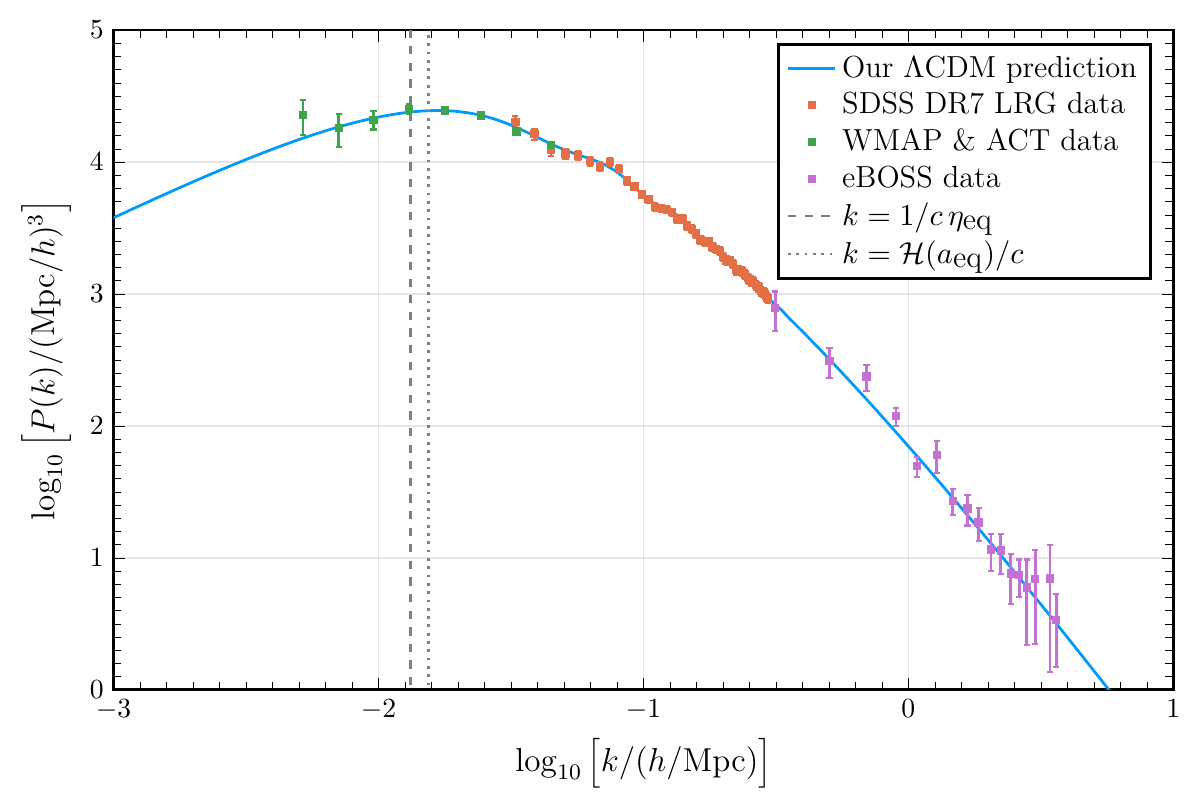
\includegraphics[width=0.7\textwidth]{../plots/power_spectrum_matter.pdf}
\caption{
	Today's matter power spectrum \eqref{eq_Pk} at $x=0$ with the Planck parameters \eqref{eq_planck2018},
	compared to data from SDSS, WMAP, ACT and eBOSS obtained from \href{https://cmb.wintherscoming.no/data/}{https://cmb.wintherscoming.no/data/}.
	The dashed line shows the $k$-value $k_\text{eq} = 1/(c \, \eta_\text{eq})$ for the perturbation mode that enters the horizon exactly at radiation-matter equality \eqref{eq_equality_radiation_matter}.
}
\label{fig_power_spectrum_matter}
\end{figure}

\Cref{fig_power_spectrum_matter} shows the computed matter power spectrum.
The agreement with data is quite good.
We see that the power spectrum turns over around
$k_\text{eq} \approx 1/c\,\eta_\text{eq} \approx \mathcal{H}(a_\text{eq})/c$:
which corresponds to modes that enter the horizon at radiation-matter equality:
\begin{itemize}
\item
Modes with $k<k_\text{eq}$ enter the horizon after radiation-matter equality.
We saw in \cref{fig_perturb_all} that the potentials change very little for such modes,
so the power spectrum \eqref{eq_Pk} roughly predicts $P \propto \Phi_0^2 k^{n_s} \propto k^{n_s} \approx k^1$,
corresponding to the line with positive slope in the logarithmic plot.

\item
Modes with $k>k_\text{eq}$ enter the horizon before radiation-matter equality.
We saw in \cref{fig_perturb_all} that the potentials for such modes change significantly from early to late times,
and increasingly for smaller-scale modes with larger $k$.
Hence, $P \propto \Phi_0^2 k^{n_s}$ rather follows what looks like a $P \propto k^{-3}$ decline,
in good agreement with the analytical $\Phi_0 \propto k^{-2}$-dependence in \cite[equation (8.71)]{dodelsonModernCosmology2021}.
\end{itemize}

\begin{figure}
\centering
\includegraphics[width=0.7\textwidth]{../plots/power_spectrum_CMB_TT.pdf} \\
\includegraphics[width=0.7\textwidth]{../plots/power_spectrum_CMB_EE.pdf} \\
\includegraphics[width=0.7\textwidth]{../plots/power_spectrum_CMB_TE.pdf}
\caption{
	Today's CMB power spectra \eqref{eq_Dl} for self- and cross-correlation between temperature and polarization with the Planck parameters \eqref{eq_planck2018},
	compared to data from Planck obtained from \href{https://cmb.wintherscoming.no/data/}{https://cmb.wintherscoming.no/data/}.
}
\label{fig_power_spectrum_cmb}
\end{figure}

\Cref{fig_power_spectrum_cmb} shows computed CMB power spectra.
The agreement with Planck's data is quite good across all $l$,
except for the highest peak being a little too low.
Let us walk through the (angular) scale dependence of the temperature self-correlation spectrum $D_l^\text{TT}$:
\begin{itemize}
\item
The relatively flat $l \lesssim 10^{1.5} \approx 30$ regime to the left of the first peak is called the Sachs-Wolfe plateau.
At these large scales, modes have entered the horizon only very recently.
They are therefore unaffected by most of the causal physics that have acted throughout the universe's lifetime,
so this plateau directly reflects the initial conditions and lets us probe inflation.
Assuming a flat primordial power spectrum that gives equal power to all scales,
the power spectrum therefore appears relatively flat in this regime.
The increase for the smallest $l \lesssim 10^1$ is caused by the late-time ISW effect,
which we explained due to the decay of gravitational potentials during dark energy-domination.

\item
The first peak at $l \approx 10^{2.3}$ represents modes whose baryonic acoustic oscillations
have reached the maximum of the first compression at recombination.
At this point, the opaque gas clears for the photons to stream away,
but they must first climb out of the wells they are compressed into,
so the temperature fluctuations appear large at this scale due to the SW effect.

\item
The first trough at $l \approx 10^{2.6}$ represents modes that have
completed one compression, begun to decompress and exactly reached the equilibrium point
where it is neither compressed nor decompressed at the time of recombination.
Thus, there are smaller differences in photons streaming towards us at these scales.
Of course, this interpretation of the SW effect is simplified, and there are other effects at play,
so there is still nonzero power at this scale -- as on all scales.

\item
The second peak at $l \approx 10^{2.7}$ represents modes that have reached
the maximum of the first decompression when the photons are released at recombination.
These photons do not have to climb out of potential wells, so they appear hot at these scales.

\item
In general, the $n$-th odd/even peak represent modes that have
undergone multiple oscillations and reached the maximum of the $n$-th compression/decompression at recombination.
Smaller-scale peaks have undergone more oscillations,
leading to more mixing of hot and cold regions from diffusion damping,
so the temperature anisotropies due to the SW effect decreases and the peaks become successively lower in amplitude.
\end{itemize}

\Cref{fig_power_spectrum_cmb} also shows the E-mode polarization self-correlation spectrum $D_l^\text{EE}$:
\begin{itemize}
\item
The polarization power spectrum has peaks where the temperature power spectrum has troughs, and vice versa.
We saw in \cref{sec_perturbations} that polarization was associated with quadrupole-like temperature fluctuations $\Theta_2$,
which is in phase with the dipole $\Theta_1$ during tight coupling \eqref{eq_perturb_tight}.
Moreover, equation \eqref{eq_radiation_velocity_overdensity} roughly relates dipoles to velocities and monopoles to overdensities,
so due to the nature of oscillations, $\Theta_0$ and $\Theta_1$ are almost perfectly out of phase.
Whereas the temperature power spectrum is largely sourced by overdensities (or $\Theta_0$),
the polarization power spectrum is therefore largely sourced by fluid velocities (or $\Theta_1 \propto \Theta_2$),
explaining why they are out of phase.

\item
There is no (nonzero) Sachs-Wolfe-like plateau in the EE-spectrum.
As the source function \eqref{eq_S} is weighted by the visibility function $\tilde{g}$,
most of the contribution comes from quadrupoles at recombination (see \cref{fig_perturb_all}) from modes entering the horizon before radiation-matter equality.
In addition, there is a smaller contribution from larger-scale modes due to photons last scattering during reionization,
which becomes visible as the small ``reionization bump'' around $l \approx 100$.

\item
The amplitude of the EE signal is much lower than the TT signal,
so anisotropies in polarization are much less pronounced than those in temperature.
\end{itemize}

\Cref{fig_power_spectrum_cmb} also shows the cross-correlation $D_l^\text{TE}$ between temperature and polarization:
\begin{itemize}
\item
From our discussion of the EE-spectrum,
we know that TE signals are dominated by correlations between density and velocity at last scattering.
Thus, very roughly speaking, its phase lies halfway between the TT and EE spectra's phases,
in other words from modes whose oscillations are closer to equilibrium instead of maximum compression or decompression at last scattering.

\item
The amplitude of the TE signal is somewhat higher than the EE signal,
but still much lower than the TT signal.
\end{itemize}

\begin{figure}
\centering
\includegraphics[width=0.49\textwidth]{../plots/power_spectrum_CMB_varying_Ωb0.pdf} \hfill
\includegraphics[width=0.49\textwidth]{../plots/power_spectrum_CMB_varying_Ωc0.pdf} \\
\includegraphics[width=0.49\textwidth]{../plots/power_spectrum_CMB_varying_Tγ0.pdf} \hfill
\includegraphics[width=0.49\textwidth]{../plots/power_spectrum_CMB_varying_Neff.pdf} \\
\includegraphics[width=0.49\textwidth]{../plots/power_spectrum_CMB_varying_As.pdf} \hfill
\includegraphics[width=0.49\textwidth]{../plots/power_spectrum_CMB_varying_ns.pdf} \\
\includegraphics[width=0.49\textwidth]{../plots/power_spectrum_CMB_varying_Yp.pdf} \hfill
\includegraphics[width=0.49\textwidth]{../plots/power_spectrum_CMB_varying_h.pdf} \\
%\includegraphics[width=0.49\textwidth]{../plots/power_spectrum_CMB_varying_z_reion_H.pdf} \\
\caption{CMB power spectra for $\Lambda$CDM models where one independent parameter is varied away from the Planck parameters \eqref{eq_planck2018} at the time, but still constrained by the relations there.}
\label{fig_power_spectrum_cmb_varying_parameters}
\end{figure}

Finally, in \cref{fig_power_spectrum_cmb_varying_parameters},
we explore the change of the CMB's TT power spectrum as we change one cosmological parameter at the time away from the Planck parameters \eqref{eq_planck2018}:
It is not trivial to think clearly about all parameter changes;
for example, changing $h$ (which intuitively corresponds to the expansion rate) would also change $\Omega_{\gamma 0} \propto T_{\gamma 0}^4/h^{2}$, and thus $\Omega_{\Lambda 0}$.
Nevertheless, let us try to understand the ``main effect'' of the most important parameters:
\begin{itemize}
\item
Increasing the baryon density $\Omega_{b0}$ amplifies the \emph{difference} between odd and even acoustic peaks.
A stupidly obvious explanation of this trend is that if there were no baryons,
there would be no baryonic acoustic oscillations
contributing to the variations in the power spectrum.
\emph{Baryon loading} refers to the effect of more baryons
increasing the gravitational force that pulls them (and their coupled photons) into dark matter wells.
This then dominates over the counteracting radiation pressure that aims to decompress the fluid,
so the odd peaks are amplified \emph{relative to} the even peaks (the third peak does not change much in an \emph{absolute} sense).
% http://background.uchicago.edu/~whu/intermediate/baryons.html|

\item
Increasing the cold dark matter density $\Omega_{c0}$ instead suppresses the entire power spectrum,
as the baryonic acoustic oscillations become less pronounced when the baryons make up less of the total matter.
\emph{Radiation driving} refers to the decay of potentials during compressions in radiation domination,
so the gravitational force that pressure fights during the following decompression is weaker,
effectively providing an external supporting force for the oscillations during radiation domination.
This effect becomes less pronounced with increasing $\Omega_{c0}$ because radiation-matter equality occurs earlier,
hence suppressing power.
Moreover, without dark matter, there would be no wells for the baryons to load,
so the fact that CMB measurements have a second (decompression) and third (compression) peak of the same height
provides good evidence that dark matter exists.

\item
Increasing today's photon temperature $T_{\gamma 0}$ increases the photon and radiation content of the universe.
This makes radiation dominate for longer,
and enhances the early-time ISW effect and radiation driving,
leading to higher peaks.
It also creates a stronger photon pressure with more violent decompressions,
leading to less damping at smaller scales.

\item
Increasing the effective number of \emph{massless} neutrinos $N_\text{eff}$
also increases the radiation content and enhances the early-time ISW effect and radiation driving,
making the first peaks higher.
However, as the neutrinos have decoupled from the baryon-photon fluid,
it does not contribute to its radiation pressure,
so power is instead suppressed at smaller scales, unlike what happened with more photons.

%\emph{Massive} neutrinos, on the other hand, are generally known to wash out structure growth.

% https://www.arxiv-vanity.com/papers/1303.5379/
% https://arxiv.org/pdf/1303.5379.pdf
% TODO: screw the peak shift, rather focus on:
%Increase neutrinos > enhance early ISW effect > amplify first peak but suppress later peaks

\item
Increasing the primordial power spectrum amplitude $A_s$
only produces an overall multiplication of the entire power spectrum through equation \eqref{eq_P_primordial}.
If there is more power on all scales to begin with,
there is more power on all scales later, as well.

\item
Increasing the spectral index $n_s>1$ gives more primordial power to modes with larger $k$.
This ``tilts'' the power spectrum so there is more power on smaller scales, and less on larger scales.
This is particularly noticeable for the Sachs-Wolfe plateau and the largest-scale modes that still resemble their primordial form.

\item
Increasing $Y_p$ increases the free electron fraction $X_e$ (see \cref{fig_free_electron_fraction}),
but \emph{decreases} the free electron number density $n_e$ (see equation \eqref{eq_free_electron_fraction_definition}).
Hence, the photon's mean free path increases,
and so does the effect of diffusion damping,
yielding a more suppressed small-scale tail.

\item
Increasing $h$ changes a lot of things and is not straightforward to reason about.
However, we see an almost overall suppression of power,
which rhymes with the intuitive picture that more rapid expansion dampens (``drags'') oscillations and hinders structure growth.
Another explanation is that more rapid expansion also means the universe is younger,
as it requires less time to expand to today's size,
so structure has less time to build up.

\item
Increasing $\Omega_{k0}$ would mainly affect the location of the first peak.
Unfortunately, we have only implemented curvature at the background level and not in the perturbations,
so we are not able to see its effects first-hand from our own program.
For example, in an open universe with $k < 0 < \Omega_{k0}$,
(initially parallel) light rays diverge,
so a temperature fluctuation would be observed on a smaller angular scale
than in a flat universe (see \cite[figure 9.14]{dodelsonModernCosmology2021}, for example).
Thus, with increasing $\Omega_{k0}$,
the power spectrum would shift to larger $l$.
The location of the peak in the measured CMB spectrum
is one of the best pieces of evidence we have
that our Universe is close to flat.
\end{itemize}

\clearpage
\section{Conclusions}

\TODO{}

\clearpage
\appendix
\section{Cosmological constraints from supernovae}
\label{sec_supernova}

In this section, we forget most of the Planck cosmological parameters \eqref{eq_planck2018} for a moment;
neglecting neutrinos by fixing $N_\text{eff}=0$ and keeping only $T_{\gamma0}$, hence fixing $\Omega_{r0}$.
Instead, we constrain the independent parameters $h$, $\Omega_{m0}$ and $\Omega_{k0}$,
and hence the dependent $\Omega_{\Lambda 0}=1-\Omega_{k0}-\Omega_{m0}-\Omega_{r0}$,
using observed supernovae luminosity distances from \cite{betouleImprovedCosmologicalConstraints2014}.
To do so, we do a Markov chain Monte Carlo (MCMC) analysis
by stepping through cosmologies with various parameters using the Metropolis-Hastings algorithm
and comparing their predicted luminosity distances to the data.

\subsection{Theory}

\subsubsection*{Cosmological distances}

From the FLRW metric \eqref{eq_flrw} and conformal time \eqref{eq_cosmic_conformal_time},
we can show how to compute distances in the universe.
Consider a photon traveling on a radial path with $d\theta = d\phi = 0$,
from emission at $(\eta,r)$ to our observation at $(\eta_0, 0)$,
along the null geodesic
\begin{equation*}
	0 = ds^2 = a^2(t) \left[ -c^2 d\eta^2 + \frac{dr^2}{1-kr^2} \right].
\end{equation*}
On the comoving grid (in $[\ldots]$), it travels the \textbf{comoving distance}
\begin{equation}
	\chi = \int_{\eta}^{\eta_0} c \, d\eta = c \, \big(\eta_0 - \eta\big) = \int_r^0 \frac{-dr}{\sqrt{1-kr^2}} = \frac{\asin\big(\sqrt{k}r\big)}{\sqrt{k}},
\label{eq_comoving_distance}
\end{equation}
so it came from the radial coordinate%
\footnote{This holds for all $k$ as $\sinc(x) = \sin x / x$ takes complex arguments, with $\sin(ix) = i \sinh x$ and $\sinc(0) = 1$.}
\begin{equation}
	r = \frac{\sin\Big(\sqrt{k}\chi\Big)}{\sqrt{k}} = \chi \sinc\Big(\sqrt{k}\chi\Big).
\label{eq_radial_coordinate}
\end{equation}

Given the observed redshift $z$ of light,
we can then compute its scale factor $a = (z+1)^{-1}$ at emission,
the corresponding conformal time \eqref{eq_cosmic_conformal_time},
the comoving distance \eqref{eq_comoving_distance}, the radial coordinate \eqref{eq_radial_coordinate}
and thus the corresponding \textbf{angular diameter distance} and \textbf{luminosity distance}
\begin{equation}
	d_A = a r
	\qquad \text{and} \qquad
	d_L = \frac{r}{a} = \frac{d_A}{a^2}.
\label{eq_distances}
\end{equation}

\subsubsection*{Statistics}

From \cite{betouleImprovedCosmologicalConstraints2014},
we have measured luminosity distances $d_{L}^\text{obs}(z_i)$ and their
corresponding measurement uncertainties $\sigma_i^\text{obs}$
for $N=31$ different redshifts $z_i$.
Given the three cosmological parameters $h$, $\Omega_{m0}$ and $\Omega_{k0}$,
we can then fit the data to corresponding theoretically predicted distances $d_L(z_i; h, \Omega_{m0}, \Omega_{k0})$.
Assuming the different measurements are Gaussian distributed and uncorrelated,
the likelihood function that rates the fit is $L \propto e^{-\chi^2/2}$, where the $\chi^2$-function is
\begin{equation}
	\chi^2(h,\Omega_{m0},\Omega_{k0}) = \sum_{i=1}^{N} \left( \frac{d_L(z_i; h, \Omega_{m0}, \Omega_{k0}) - d_{L}^\text{obs}(z_i)}{\sigma_i^\text{obs}} \right)^2.
\label{eq_chi2}
\end{equation}

The Metropolis-Hastings algorithm steps through various combinations of $\mathbf{p} = (h,\Omega_{m0},\Omega_{k0})$ in parameter space, measuring their likelihood $L(\mathbf{p})$.
Each iteration $i$, it randomly shifts the parameters from their current values with a normal distribution,
and then records their new values as a random sample of their probability distribution with probability $\min\big\{L_{i+1}/L_i, 100\%\big\}$.

By the central limit theorem, once the algorithm has gathered many samples $\mathbf{p}_i$,
they should scatter around the \emph{best fit}
with maximum $L(\mathbf{p}_\text{best}) = \max\{L(\mathbf{p}_i)\}$
like a multivariate Gaussian with the same dimension $D$ as the parameter space.
We can then produce \emph{confidence regions} for the parameters
by identifying contours that enclose a given fraction $F$ of the samples.
For a multivariate Gaussian distribution, a fraction $F$ is enclosed by an ellipsoid
for which
\begin{equation}
	\chi^2_i - \chi^2_\text{best} < q_{\chi^2_D}(F),
\label{eq_confidence_region}
\end{equation}
where $q_{\chi^2_D}(F)$ is the inverse cumulative distribution function of the $\chi^2$-distribution with $D$ degrees of freedom.
We have $D=3$ independent parameters, and look for standard $68.3\%$ and $95.4\%$ confidence regions
with $q_{\chi^2_3}(68.3\%) \approx 3.53$ and $q_{\chi^2_3}(95.4\%) \approx 8.00$.

\subsection{Implementation}

\begin{itemize}
	\item We roll our own homemade Metropolis-Hastings algorithm.
	      It takes a function that computes the likelihood $L(\mathbf{p})$ for a set of parameters $\mathbf{p}$.
	      Unless specified explicitly, it sets step sizes of the parameters as a proportion of their lower and upper bounds,
		  and adaptively scales them if the algorithm accepts samples at a rate too far from the ``optimal'' acceptance rate around $25\%$ \cite{gelmanWeakConvergenceOptimal1997}.
		  The algorithm can run multiple chains from different initial parameter guesses,
		  each with a requested number of (accepted) samples after removing a given number of burn-in samples.
	\item We exclude parameters outside their specified bounds by assigning $L=0$ to them.
	\item As mentioned in \cref{sec_background_cosmology_theory},
	      our implementation of the background cosmology parametrized by the scale factor
	      \textbf{cannot handle cosmologies with turnaround} $\dot{a} = 0$.
	      These cosmologies can arise now that we allow $\Omega_{k0} \neq 0$,
	      for example with $\Omega_{r0}=0$, $\Omega_{m0} = 0.2$ and $\Omega_{k0} = -0.9$ and $\Omega_{\Lambda0} = 1.7$.
	      We identify such cosmologies as described in \cref{sec_background_cosmology_implementation}, and exclude them by setting $L=0$.
\end{itemize}

\subsection{Results}

\begin{figure}[!b]
	\centering
	\includegraphics[scale=0.7]{../plots/supernova_distance.pdf}
	\caption{Observed and predicted luminosity distances \eqref{eq_distances} from \cite{betouleImprovedCosmologicalConstraints2014} and the Planck cosmology \eqref{eq_planck2018}.}
	\label{fig_luminosity_distances}
\end{figure}

\Cref{fig_luminosity_distances} shows observed and predicted luminosity distances from the Planck 2018 cosmology \eqref{eq_planck2018}.
The prediction steers wide of most error bars, so the agreement is not very good!
This shows that supernovae are promising sources for generating orthogonal constraints on cosmological parameters complementary to the widely ``accepted'' Planck values, for example.
The plot also shows the much better agreement from the best fit parameters that we find next.

\begin{figure}[b]
	\centering
	\includegraphics[scale=0.7]{../plots/supernova_hubble.pdf}
	\includegraphics[scale=0.7]{../plots/supernova_omegas.pdf}
	\caption{%
		Probability distribution of today's reduced Hubble parameter $h$,
		and confidence regions \eqref{eq_confidence_region} for $\Omega_{m0}$ and $\Omega_{\Lambda0}$,
		from $10 \times 10000$ Metropolis-Hastings samples with $L \propto e^{-\chi^2/2}$ and the $\chi^2$ sum \eqref{eq_chi2},
		comparing predicted luminosity distances \eqref{eq_distances} to observations from \cite{betouleImprovedCosmologicalConstraints2014}.
		The algorithm restricts the parameters to the prior bounds $h \in [0.5, 1.5]$, $\Omega_{m0} \in [0, 1]$ and $\Omega_{k0} \in [-1, +1]$, and accordingly (with negligible radiation today) $\Omega_{\Lambda0} \in [-1, 2]$.
	}
	\label{fig_supernova_mcmc}
\end{figure}

\Cref{fig_supernova_mcmc} shows our MCMC constraints on $h$, $\Omega_{m0}$ and $\Omega_\Lambda$,
from the prior bounds $h \in [0.5, 1.5]$, $\Omega_{m0} \in [0, 1]$ and $\Omega_{k0} \in [-1, +1]$
that accommodate a wide region around the Planck values \eqref{eq_planck2018}, for example.
In addition, curved universes with a turnaround $\dot{a} = 0$ are forbidden
(\cite[Figure 11]{amanullahSpectraLightCurves2010} shows that such cosmologies are disconnected from the best fit regions, anyway).

Note that the constraint in the $\Omega_{m0}$-$\Omega_{\Lambda0}$-plane is highly orthogonal to the line of flat universes,
so supernova data can give good constraints when combined with some other argument in favor of flatness, for example.
Our best fits for $\Omega_{m0}$ and $\Omega_{\Lambda0}$ agrees relatively well with a similar analysis in \cite[Fig. 15]{betouleImprovedCosmologicalConstraints2014}.
Our Hubble parameter is significantly larger than Planck's and exemplifies the Hubble tension.

\clearpage

\section{To-do list}

\begin{itemize}
\item \TODO{use article template?}

\item \TODO{list with radiation driving, baryon loading, diffusion damping. mention in perturbation section, so I can refer back here?}
\end{itemize}

\clearpage
%\bibliography{report.bib}
\printbibliography

\end{document}
